\documentclass[openright,twoside,10pt]{book}
\usepackage[b5paper,left=2cm,top=2.5cm,right=1.5cm,bottom=2.5cm]{geometry} 
\usepackage[spanish]{babel} % espanol
\usepackage[utf8]{inputenc} % acentos sin codigo
\usepackage{graphicx} % gráficos
\usepackage{pdflscape}
\usepackage{fancyvrb}
\usepackage{fancyhdr}
\usepackage{wrapfig}


%% Mis paquetes
\usepackage{subcaption}
\usepackage{enumerate}
\usepackage[acronym, toc]{glossaries}
\usepackage{multicol}
\usepackage{multirow}
\usepackage{booktabs}
\usepackage[dvipsnames]{xcolor}
\usepackage{ragged2e}
\usepackage{tabularx}
\usepackage{ifthen} % para la tabla de riesgos
%\usepackage{hyperref}
\usepackage{longtable}
\usepackage{float}
\usepackage{eurosym} % para el euro
\usepackage{listings}
\usepackage{framed}
\usepackage{newfloat}
\usepackage{caption}
\usepackage{xurl}
\usepackage[colorlinks]{hyperref}

\hypersetup{
	allcolors = {blue}
}

\usepackage[table,xcdraw]{xcolor} % Para colores en tablas
\usepackage{array} % Para mayor control de columnas
\usepackage{pgfgantt}
\usepackage{colortbl}
\usepackage{array}
\usepackage{enumitem}
\usepackage{xcolor}




\renewcommand{\arraystretch}{1.45}

\definecolor{redrisk}{RGB}{255, 59, 48}     % Rojo intenso
\definecolor{orangerisk}{RGB}{255, 149, 0}  % Naranja brillante
\definecolor{yellowrisk}{RGB}{255, 204, 0}  % Amarillo vibrante
\definecolor{greenrisk}{RGB}{52, 199, 89}   % Verde esmeralda
\definecolor{bluerisk}{RGB}{0, 122, 255}    % Azul eléctrico
\definecolor{purplerisk}{RGB}{175, 82, 222} % Púrpura intenso\\
\definecolor{lightgray}{RGB}{230,230,230}



\DeclareFloatingEnvironment[fileext=frm,placement={!ht},name=Fragmento de código]{codefragment}

\captionsetup[codefragment]{labelfont=bf}

\setlength{\parskip}{10pt plus 1pt minus 1pt}

\newcolumntype{L}{>{\raggedright\arraybackslash}X} % for ragged-right material
\newcolumntype{Z}{>{\hsize=\dimexpr2\hsize-29\tabcolsep+\arrayrulewidth\relax}X}
\newcolumntype{P}{p{0.22\textwidth}L p{0.78\textwidth}L}
%\newcolumntype{C}{>{\centering\arraybackslash}X}   % for centered material

\extrarowheight = +0.5ex

 % creación del glosario de términos
\makeglossaries % glosario de términos
\newglossaryentry{termino}
{
    name=término,
    description={Descripción}
}

\newacronym{ii}{II}{Ingniería en Informática}

\setglossarystyle{altlisthypergroup}

 % aqui definimos el encabezado de las paginas pares e impares.
\rhead[]{}

\renewcommand{\headrulewidth}{0.5pt}

% aqui definimos el pie de pagina de las paginas pares e impares.
\rfoot[\thepage]{\thepage}
\cfoot[]{}
\renewcommand{\footrulewidth}{0pt}

%redefino el verbatim
%\renewenvironment{verbatim}{\begin{Verbatim}[frame=single,fontsize=\small]}{\end{Verbatim}}


% aqui definimos el encabezado y pie de pagina de la pagina inicial de un capitulo.
\fancypagestyle{plain}{
\fancyhead[R]{}
\fancyfoot[C]{}
\fancyfoot[R]{\thepage}
\renewcommand{\headrulewidth}{0.5pt}
\renewcommand{\footrulewidth}{0pt}
}

\pagestyle{fancy} % seleccionamos un estilo



\renewcommand\spanishtablename{Tabla}
\renewcommand{\spanishlisttablename}{Lista de Tablas} 
\renewcommand{\spanishlistfigurename}{Lista de Figuras} 

\date{2024-2025}
\author{Hugo López Álvarez}

\title{Diseño de un modelo neuronal para la detección y la clasificación de intrusiones en redes informáticas}


\raggedbottom
\begin{document}

\begin{titlepage}

\begin{center}
\vspace*{-0.5in}
\begin{figure}[htb]
\begin{center}

\includegraphics[width=5cm]{./img/uva}
\end{center}
\end{figure}
%\begin{large}
%\textbf{Universidad de Valladolid}
%\end{large}

\vspace*{0.3in}
\huge
{\fontfamily{phv}\selectfont Escuela de Ingeniería Informática}
\\
\vspace*{0.5in}
\large
{\fontfamily{phv}\selectfont \textbf{\textsc{\textsc{TRABAJO FIN DE GRADO}}}}

	
\vspace*{0.2in}
\fontfamily{phv}\selectfont Grado en Ingeniería Informática\\
\fontfamily{phv}\selectfont Mención en Tecnologías de la Información\\
\vspace*{0.8in}
\huge
{\fontfamily{phv}\selectfont\textbf{Diseño de un modelo neuronal para la detección y la clasificación de intrusiones en redes informáticas}}
\vspace*{1in}
\begin{large}
\begin{flushright}
Alumno:\\\textbf{Hugo López Álvarez}\\
\vspace*{0.3in}
Tutor:\\ \textbf{Diego García Álvarez}\\
\end{flushright}
\end{large}
\end{center}

\end{titlepage}

\newpage
\mbox{}	
\thispagestyle{empty} % para que no se numere esta página

\chapter*{}
\pagenumbering{Roman} % para comenzar la numeración de paginas en números romanos
\begin{flushright}
\textit{%Dedicatoria,\\
...}
\end{flushright}

\chapter*{Agradecimientos} % si no queremos que añada la palabra "Capitulo"
\addcontentsline{toc}{chapter}{Agradecimientos} % si queremos que aparezca en el índice
\markboth{AGRADECIMIENTOS}{AGRADECIMIENTOS} % encabezado 

...

\chapter*{Resumen} % Se pone * si no queremos que añada la palabra "Capitulo"
\addcontentsline{toc}{chapter}{Resumen} % si queremos que aparezca en el índice
\markboth{RESUMEN}{RESUMEN} % encabezado
\begin{flushleft}
Resumen

\end{flushleft}


\chapter*{Abstract} % Se pone * si no queremos que añada la palabra "Capitulo"
\addcontentsline{toc}{chapter}{Abstract} % si queremos que aparezca en el índice
\markboth{ABSTRACT}{ABSTRACT} % encabezado
\begin{flushleft}

Abstract

\end{flushleft}

\tableofcontents % indice de contenidos

\cleardoublepage
\addcontentsline{toc}{chapter}{Lista de figuras} % para que aparezca en el indice de contenidos
\listoffigures % indice de figuras

\cleardoublepage
\addcontentsline{toc}{chapter}{Lista de tablas} % para que aparezca en el indice de contenidos
\listoftables % indice de tablas

\clearpage

\printglossary[title=Glosario de términos, toctitle=Glosario de términos]
\glsaddall
\clearpage

\printglossary[type=\acronymtype]

\chapter{Introducción}\label{cap.introduccion}
\pagenumbering{arabic} % para empezar la numeración con números
Este documento corresponde con la memoria del Trabajo de Fin de Grado (TFG) del Grado en Ingeniería Informática de la Escuela de Ingeniería Informática (EII) de la Universidad de Valladolid (UVa). Este trabajo se centra en el diseño e implementación de un modelo neuronal capaz de detectar intrusiones en una red informática. El modelo está dividido en dos niveles de clasificación, un modelo de clasificación binaria que clasifica las conexiones como benignas o malignas, y un modelo de clasificación multiclase que recibe como entradas las conexiones clasificadas por el modelo binario como malignas. Este último modelo distingue en nueve tipos diferentes de intrusiones las conexiones que recibe, es decir, trata de determinar el tipo de intrusión. El uso de redes neuronales para la detección de intrusiones permite identificar patrones complejos y no lineales en el tráfico de red, mejorando la capacidad de detectar ataques desconocidos o sofisticados. Además, las redes neuronales pueden adaptarse y aprender continuamente a partir de nuevos datos, aumentando su precisión con el tiempo.

%La principal ventaja de utilizar un modelo neuronal para la detección de intrusiones en una red, frente a los algoritmos tradicionales (como firmas basadas en reglas o análisis estadísticos), radica en su capacidad para aprender patrones complejos y no lineales en los datos, lo que le permite identificar amenazas desconocidas o variantes de ataques existentes (zero-day attacks). Mientras que los métodos tradicionales dependen de reglas predefinidas y actualizaciones manuales para detectar intrusiones (limitándose a ataques conocidos), las redes neuronales pueden analizan grandes volúmenes de tráfico de red, detectando anomalías sutiles y correlaciones ocultas mediante capas de abstracción.

\section{Contexto} \label{sec.exp-problema}
En la actualidad, los sistemas informáticos reciben muchos más ataques de denegación de servicio y de intrusión que hace unos años, esto se debe en parte a los avances en los modelos de Inteligencia Artificial (IA). Los sistemas informáticos enfrentan actualmente graves amenazas debido al uso malintencionado de la IA por parte de ciberdelincuentes. Una de las principales problemáticas es la automatización de ataques, donde herramientas basadas en IA permiten ejecutar campañas de ataques informáticos con mayor precisión y escala. Estas IAs pueden generar mensajes convincentes, imitar patrones de comportamiento legítimos y evadir medidas de seguridad tradicionales, lo que incrementa la frecuencia y sofisticación de los ataques. 

Otro desafío crítico es la explotación de vulnerabilidades mediante IA, que acelera la identificación de fallos en sistemas sin intervención humana. Existen algoritmos de aprendizaje automático (\textit{Machine Learning}, ML) que analizan grandes volúmenes de datos para descubrir brechas de seguridad en tiempo récord, facilitando ataques dirigidos incluso contra infraestructuras críticas como hospitales. Por estos motivos, la ciberseguridad es una tema de actualidad del que cada vez más se habla con más frecuencia incluso en la prensa general o económica \cite{rundle2024ai}.

La IA también complica la defensa, ya que los sistemas de detección tradicionales no siempre pueden anticipar tácticas adaptativas generadas por algoritmos hostiles. Esto obliga a las organizaciones y empresas a invertir en soluciones de IA defensiva, como sistemas de respuesta autónoma. Sin embargo, esto genera una carrera tecnológica desigual donde actores maliciosos aprovechan herramientas accesibles y de bajo costo. La falta de regulación global agrava este escenario, dificultando la mitigación de riesgos asociados.  

Además, los modelos neuronales son adaptativos: mejoran su precisión con el tiempo al entrenarse con nuevos datos, lo que es crucial en entornos dinámicos donde los ciberataques evolucionan rápidamente. Por ejemplo, pueden distinguir entre comportamientos legítimos inusuales (como un empleado accediendo a recursos fuera de horario) y actividades maliciosas (como filtración de datos), reduciendo falsos positivos. En cambio, los enfoques tradicionales suelen ser rígidos y requieren ajustes manuales frecuentes para mantener su eficacia.

Sin embargo, el uso de modelos nueronales para la defensa de los sistemas conlleva grandes desafíos, como la necesidad de grandes conjuntos de datos etiquetados y recursos computacionales intensivos. Aun así, en escenarios donde la sofisticación de los ataques supera las capacidades de detección convencionales, los modelos neuronales representan un salto cualitativo en proactividad y escalabilidad. 



\section{Motivación} \label{sec.motivacion}

La principal motivación, que impulsó el desarrollo de este proyecto es facilitar la detección de ataques en redes informáticas, que tantas complicaciones está generando a los encargados de la administración de estos sistemas. Para complir con esta motivación, se decidió implementar un modelo neuronal que cumpliese con estos requisitos.

Durante la formación universitaria en el Grado en Ingeniería Informática,los alumnos
de la mención de tecnologías de la información, aprenden a administrar grandes sistemas de computación en aspectos como: la seguridad, la garantía de la información, la evaluación de dichos sistemas y el almacenamiento de los datos. Además de contener formación sobre ciertos componentes de desarrollo de software. La falta de formación en algunos aspectos de la IA en dicha mención, desemboca en una de las grandes motivaciones académicas para desarrollar este proyecto, como es la familiarización con las técnicas de ML, en concreto de las redes neuronales, como herramientas útiles.

 
\section{Objetivos del proyecto} \label{sec.objetivos-pro}
En esta sección se listan los objetivos del proyecto, que constituyen las metas específicas, medibles, alcanzables, relevantes y con plazos definidos que se persiguen con la ejecución del mismo. Dichos objetivos describen los resultados concretos que se espera lograr al finalizar el proyecto y proporcionan un marco de referencia para la planificación, la ejecución, el seguimiento y la evaluación de su progreso.

\begin{enumerate}
	\item Diseñar e implementar un modelo capaz de detectar intrusiones en redes informáticas y proporcionar una clasificación previa de la intrusión.
	\item Desarrollar modelos de detección que han de ser modelos neuronales.
	\item Evaluar y comparar los modelos generados con un dataset real y complejo.
\end{enumerate}

\section{Objetivos académicos} \label{sec.objetivos-aca}
En esta sección se enumeran los objetivos académicos del presente estudio, los cuales representan las metas específicas, susceptibles de evaluación, realizables, pertinentes para el ámbito del conocimiento, que se pretenden alcanzar a través del desarrollo de este proyecto. 

\begin{enumerate}
	\item Comprender el funcionamiento de los modelos neuronales a través de \texttt{PyTorch} y las métricas de evaluación.
	\item Asimilar las características de varios tipos de modelos neuronales existentes.
	\item Descubrir el potencial de las redes neuronales para optimizar y mejorar las tecnologías de la información, incluyendo la ciberseguridad de los sistemas.

\end{enumerate}


\section{Estrucutra de la memoria} \label{sec.estr-memoria}

Este trabajo fin de grado se estructura de la siguiente manera:
\begin{description}
\item[Capítulo 2 Metodología:] En este capítulo se definen cuales son las fases de la metodología CRISP-DM que se utiliza como metodología y modelo de proceso para el diseño y evaluación de los modelos neuronales para la detección de intrusiones. Se describe la aplicación de cada una de las seis fases al contexto específico del desarrollo de modelos neuronales.

\item[Capítulo 3 Planificación:] Este capítulo presenta la planificación del proyecto. Se definen los recursos necesarios, se identifican las tareas principales, se estiman los plazos y se establece el cronograma. También se aborda la gestión de riesgos inicial y la asignación de roles.

\item[Capítulo 4 Entendimiento del problema:] En este capítulo se describe el problema que el proyecto busca abordar. Se presenta el contexto, la relevancia y los objetivos generales.

\item[Capítulo 5 Entendimiento de los datos:] Este capítulo se dedica a la exploración y comprensión del conjunto de datos utilizado para el entrenamiento y evaluación de los modelos desarrollados. Se describe la fuente, el formato, el tamaño y las variables de los datos. Se presenta un análisis exploratorio para identificar patrones, problemas de calidad y la distribución de las variables.

\item[Capítulo 6 Modelos:] En este capítulo se detallan los modelos de redes neuronales desarrollados y entrenados. Se describe la arquitectura, la justificación de su elección, los hiperparámetros, la función de pérdida y el optimizador. Se incluye la estrategia de entrenamiento y las métricas de evaluación.

\item[Capítulo 7 Evaluación:] Este capítulo se centra en la evaluación final de los modelos entrenados. Se describe el conjunto de datos de prueba, el proceso de evaluación, la presentación de los resultados de las métricas y el análisis de las fortalezas y debilidades de los modelos.

\item[Capítulo 8 Despliegue:] Este capítulo aborda la fase de despliegue de los modelos entrenados. Se describe la integración en un entorno operativo, las consideraciones técnicas, los posibles desafíos y las estrategias de monitorización y mantenimiento. Debido a la diversidad de entornos existentes en los que se puede realizar el despliegue, se comentarán los pasos generales que habría que seguir para desplegar los modelos en un entorno de producción real, sin entrar en profundidad.

%\item[Capítulo 9 Tecnologías utilizadas:] En este capítulo se listan y describen las tecnologías de software y hardware empleadas en el proyecto. Se incluyen lenguajes de programación, bibliotecas de aprendizaje automático, herramientas de visualización y plataformas de seguimiento de experimentos.

%\item[Capítulo 10 Seguimiento del proyecto:] Este capítulo describe cómo se ha realizado el seguimiento del progreso del proyecto. Se definen los indicadores clave de rendimiento, las metodologías de seguimiento, las herramientas de gestión y los mecanismos para la identificación y resolución de desviaciones.

\item[Capítulo 9 Conclusiones:] En este capítulo final se presentan las conclusiones del proyecto. Se resumen los principales hallazgos, se evalúa el cumplimiento de los objetivos académicos, se discuten las implicaciones de los resultados, las limitaciones y las posibles líneas de trabajo futuro.
\end{description}


\chapter{Metodología}\label{cap.metologia}

En este capítulo se explica la metodología CRISP-DM (Cross-Industry Standard Process for Data Mining), que se utiliza en el desarrollo del resto del proyecto para alcanzar los objetivos propuestos.

La adopción de metodologías estructuradas es fundamental en el desarrollo de proyectos informáticos, puesto que proporcionan un marco sistemático para garantizar la calidad, eficiencia y trazabilidad del proyecto. En particular, metodologías como CRISP-DM, permiten: alinear objetivos técnicos con necesidades de negocio,reducir riesgos mediante fases iterativas y documentadas, y facilitar la colaboración entre equipos multidisciplinares.

Según algunos estudios, los proyectos que utilizan metodologías estandarizadas incrementan un 35\% su probabilidad de éxito, frente a aproximaciones \textit{ad-hoc}, al minimizar desviaciones en costes y plazos \cite{chapman2000crisp}. En el ámbito de la ciberseguridad, donde los requisitos legales y técnicos son críticos, este enfoque metodológico resulta indispensable para asegurar soluciones robustas y auditables

\section{CRISP-DM}
La metodología CRISP-DM, es un marco de trabajo estandarizado para guiar proyectos de minería de datos y aprendizaje automático. Su estructura cíclica y flexible la hace aplicable en diversos dominios, desde marketing hasta ciberseguridad. Está compuesta por las siguientes fases:

\textbf{1. Comprensión del negocio:} La primera fase de CRISP-DM establece los cimientos estratégicos del proyecto mediante un proceso de alineación entre los objetivos técnicos y las necesidades organizacionales. Para lograr establecer los cimientos, se lleva a cabo un análisis exhaustivo del contexto empresarial para identificar los problemas clave que el proyecto debe abordar, así como las oportunidades de mejora que podrían aprovecharse. Se realiza un proceso de recopilación y documentación de requisitos que involucra a todas las partes interesadas relevantes. El resultado de esta fase es una definición precisa del alcance del proyecto, que incluye no solo los objetivos cuantificables sino también los criterios de éxito que permitirán evaluar el impacto real de la solución propuesta. Además, se establecen las limitaciones operativas y estratégicas que condicionarán el desarrollo del proyecto, asegurando que todas las fases posteriores se ejecuten dentro de un marco bien definido y alineado con las prioridades organizacionales.


\textbf{2. Comprensión de los datos:} Esta fase se centra en el análisis detallado de los datos disponibles para el proyecto, con el objetivo de evaluar su idoneidad y calidad para abordar los problemas identificados en la fase anterior. Este proceso implica un examen minucioso de las diversas fuentes de información, su estructura y sus características fundamentales. Durante esta etapa, se identifican y documentan aspectos críticos como la complejidad de los datos, la presencia de posibles sesgos y la representatividad de la información en relación con los objetivos del proyecto. La comprensión profunda de los datos permite anticipar desafíos potenciales y establecer estrategias adecuadas para su tratamiento en fases posteriores. Además, esta fase proporciona perspectivas que pueden influir en decisiones técnicas importantes, como la selección de algoritmos o el diseño de características. El resultado es un conocimiento del potencial y las limitaciones de los datos disponibles, que sirve como base para las transformaciones que se realizan en la siguiente fase.

\textbf{3. Preparación de los Datos:} Se trata de una fase crítica donde los datos brutos se transforman en un conjunto adecuado para modelado. Esta etapa implica una serie de operaciones fundamentales que garantizan la calidad y consistencia de los datos que alimentan a los modelos analíticos. Las actividades realizadas en esta fase son cruciales para el éxito del proyecto, ya que determinan en gran medida la capacidad de los algoritmos para extraer patrones significativos y generar resultados confiables. Se aplican técnicas especializadas para abordar problemas comunes en los datos, asegurando que la información sea representativa, completa y se encuentre adecuadamente estructurada para los análisis posteriores. Cualquier deficiencia en la preparación de los datos puede comprometer significativamente la efectividad de las siguientes fases. Al finalizar este proceso, se obtiene un conjunto de datos optimizado que conserva la esencia de la información original mientras elimina ruido y distorsiones que podrían afectar negativamente a los resultados del modelado.


\textbf{4. Modelado:} Constituye el núcleo técnico del proceso CRISP-DM, donde se desarrollan y evalúan los algoritmos diseñados para extraer conocimiento de los datos preparados. Esta etapa comienza con la selección cuidadosa de las técnicas de modelado más apropiadas para los objetivos específicos del proyecto y las características de los datos disponibles. Durante el proceso de modelado, se exploran diferentes enfoques algorítmicos, ajustando meticulosamente sus parámetros para optimizar su rendimiento. En esta fase se incluyen procesos de validación diseñados para garantizar que los modelos desarrollados sean robustos y generalizables, capaces de mantener su efectividad cuando se enfrenten a datos nuevos y no vistos previamente. El modelado es un proceso iterativo que puede requerir volver a fases anteriores para refinar la preparación de datos o incluso reconsiderar algunos aspectos del planteamiento inicial del problema. El resultado de esta fase es uno o varios modelos validados que cumplen con los criterios de calidad establecidos y están listos para su evaluación en el contexto de los objetivos empresariales definidos inicialmente.  

\textbf{5. Evaluación:} Esta fase representa un examen exhaustivo de los modelos desarrollados, contrastando su desempeño técnico con los objetivos empresariales establecidos en la primera fase del proyecto. Este proceso va más allá de las métricas estadísticas tradicionales para incorporar una valoración del impacto potencial de la solución propuesta. Durante la evaluación, se analiza minuciosamente la capacidad de los modelos para resolver el problema de negocio original, considerando tanto su precisión técnica como su aplicabilidad práctica en el contexto organizacional. Se identifican y documentan las limitaciones de los modelos, así como los posibles riesgos asociados a su implementación. Esta fase también incluye la validación de los resultados con las partes interesadas clave, asegurando que la solución cumpla con las expectativas y requisitos operativos. La evaluación termina con una decisión fundamentada sobre la idoneidad de los modelos para su implementación, junto con recomendaciones para su posible mejora o adaptación a escenarios futuros. También se valida su robustez en escenarios realistas.

\textbf{6. Despliegue:} Se trata de la fase final de CRISP-DM, esta se centra en la transición del modelo analítico desde un entorno de desarrollo a un sistema operativo donde pueda generar valor tangible para la organización. Este proceso implica una serie de actividades cuidadosamente planificadas que garantizan la integración efectiva de la solución en los procesos empresariales existentes. El despliegue incluye aspectos técnicos como la implementación de la infraestructura necesaria, el desarrollo de interfaces adecuadas y la creación de mecanismos de monitoreo continuo. También se ha de tener en cuenta la capacitación de los usuarios finales y la documentación exhaustiva de la solución, asegurando su adopción efectiva y su uso óptimo. La fase de despliegue también establece procesos para el mantenimiento y actualización periódica del modelo, puesto que las soluciones analíticas requieren evolución continua para mantener su relevancia y efectividad. Como en el resto de metodologçias, se implementan mecanismos para medir el impacto real de la solución una vez en producción, cerrando el ciclo al proporcionar retroalimentación valiosa que puede ser la base de futuros proyectos analíticos.

Como se ha explicado, CRISP-DM es una metodología iterativa, esto significa que los resultados de fases posteriores pueden revelar la necesidad de ajustes en etapas anteriores (como recolectar más datos o redefinir objetivos). Su enfoque estructurado minimiza riesgos y maximiza el valor entregado, siendo especialmente útil en proyectos complejos donde la alineación entre técnica y negocio es esencial.

\section{INSERTAR IMǴEN METODOLOGÍA}
\begin{figure}[htbp]
    \centering
    \includegraphics[width=0.8\textwidth]{./img/metodologia/crispdm.jpeg}
    \caption{Esquema del ciclo CRISP-DM estándar.}
    \label{fig:CRISP-DM}
\end{figure}

\chapter{Planificación}
Este capítulo aborda la organización detallada de un Trabajo de Fin de Grado, cubriendo desde su diseño inicial hasta la implementación y el seguimiento durante su desarrollo. Una planificación rigurosa resulta fundamental para sentar las bases del proyecto, ya que permite definir con claridad los objetivos, los recursos necesarios, los plazos de entrega y las actividades clave para alcanzar los resultados esperados.

En primer lugar, se establece una planificación temporal preliminar, donde se estiman los tiempos requeridos para cada etapa. Este cronograma se estructura en torno a las fases de la metodología CRISP-DM, complementadas con etapas específicas propias de un Trabajo de Fin de Grado. A continuación, se realiza un análisis de riesgos exhaustivo, evaluando tanto la probabilidad como el impacto de cada posible contingencia.

Además, se elabora un presupuesto detallado para las tareas del proyecto, abordado desde dos perspectivas. Por un lado, se incluye una estimación realista de los costes asociados a la ejecución del trabajo en el ámbito académico. Por otro lado, se plantea una proyección teórica de los gastos que implicaría un proyecto equivalente en un contexto profesional.

Por último, se contrasta la planificación inicial con el desarrollo real del trabajo, lo que permite evaluar posibles desviaciones y los aprendizajes obtenidos durante el proceso.

\section{Planificación temporal}

La planificación temporal constituye un elemento fundamental en la ejecución de un proyecto fin de grado, ya que permite estructurar de manera sistemática todas las actividades necesarias para alcanzar los objetivos propuestos. En el contexto de un trabajo académico que combine el desarrollo de software con una metodología de investigación, como es el caso de CRISP-DM para el proceso analítico y SCRUM para la gestión del proyecto, una adecuada planificación garantiza la distribución equilibrada del tiempo disponible entre las distintas fases del trabajo. Esta organización temporal resulta especialmente relevante cuando se deben coordinar aspectos teóricos, desarrollo técnico y validación de resultados, asegurando que cada componente reciba la atención necesaria sin comprometer la calidad global del proyecto.

El empleo de un diagrama de Gantt como herramienta de planificación ofrece ventajas significativas para visualizar la secuencia de actividades y su superposición temporal. Este tipo de representación gráfica facilita la identificación de hitos críticos y dependencias entre tareas, aspectos particularmente importantes cuando se combinan metodologías diferentes como CRISP-DM y SCRUM. La primera, con sus fases bien definidas, proporciona la estructura para el desarrollo del núcleo analítico del proyecto, mientras que SCRUM, con sus sprints iterativos, permite adaptar el trabajo a los descubrimientos que vayan surgiendo durante la investigación. La integración de ambas aproximaciones en un único cronograma exige una cuidadosa coordinación que el diagrama de Gantt ayuda a materializar de forma clara y comprensible.


\begin{figure}[h]
\centering
\makebox[\linewidth][c]{%  % Centrado mejorado
\begin{ganttchart}[
    x unit=0.15cm,         % Aumentado para ocupar más ancho
    y unit title=0.8cm,
    y unit chart=0.6cm,
    hgrid,
    vgrid={*{1}{dotted}},
    title/.style={draw=none},
    title label font=\footnotesize,
    bar/.style={fill=blue!30, rounded corners=2pt},
    bar height=0.6,
    group/.style={draw=black, fill=blue!10},
    milestone/.style={fill=red, rounded corners=2pt},
    bar label font=\scriptsize,
    group label font=\small,
    milestone label font=\scriptsize,
    expand chart=\linewidth  % Ocupa todo el ancho disponible
]{1}{90}
    % Título principal centrado sobre semanas
    \gantttitle{Diagrama de Gantt del Proyecto}{90} \\
    
    % Cabecera de semanas (13 semanas para 90 días)
    \gantttitlelist{1,2,3,4,5,6,7,8,9,10,11,12,13}{7} \\
    
    % Fases y tareas (igual que antes pero ajustadas visualmente)
    \ganttgroup{1. Comprensión Negocio}{1}{10} \\
    \ganttbar{1.1 Definición objetivos}{1}{5} \\
    \ganttbar{1.2 Análisis requisitos}{6}{10} \\
    
    \ganttgroup{2. Comprensión Datos}{11}{20} \\
    \ganttbar{2.1 Recopilación datos}{11}{15} \\
    \ganttbar{2.2 Análisis exploratorio}{16}{20} \\
    
    \ganttgroup{Sprint 1: Preparación}{21}{35} \\
    \ganttbar{3.1 Limpieza datos}{21}{25} \\
    \ganttbar{3.2 Feature engineering}{26}{30} \\
    \ganttbar{3.3 Normalización}{31}{35} \\
    \ganttmilestone{Hito 1}{35} \\
    
    \ganttgroup{Sprint 2: Modelado}{36}{60} \\
    \ganttbar{4.1 Selección algoritmos}{36}{40} \\
    \ganttbar{4.2 Entrenamiento inicial}{41}{50} \\
    \ganttbar{4.3 Ajuste parámetros}{51}{60} \\
    \ganttmilestone{Hito 2}{60} \\
    
    \ganttgroup{Sprint 3: Evaluación}{61}{80} \\
    \ganttbar{5.1 Validación cruzada}{61}{65} \\
    \ganttbar{5.2 Pruebas rendimiento}{66}{70} \\
    \ganttbar{5.3 Análisis resultados}{71}{80} \\
    \ganttmilestone{Hito 3}{80} \\
    
    \ganttgroup{6. Documentación}{81}{90} \\
    \ganttbar{6.1 Redacción memoria}{81}{85} \\
    \ganttbar{6.2 Preparación defensa}{86}{90} \\
    \ganttmilestone{Entrega Final}{90}
\end{ganttchart}
}
\caption{Diagrama de Gantt con planificación semanal y detalle diario}
\label{fig:gantt}
\end{figure}

\section{Gestión de riesgos}
\section{Estimación de costes}
\subsection{Costes materiales}
\subsection{Costes humanos}\label{cap.req-planificacion}

\chapter{Entendimiento del problema}\label{cap.ent.problema}
En este capítulo se trata el entendimiento del problema. Tal y como se comenta en el capítulo dos, es la fase inicial de la metología CRISP-DM. A continuación, se alinean los objetivos técnicos con las necesidades del negocio y con el problema a resolver. Se definen requisitos, se identifican métricas de éxito y se trata de dar comprensión sobre el contexto organizacional.


\section{¿Qué es un ataque a un sistema informático?}
Un ataque a un sistema informático constituye una acción deliberada y no autorizada que explota vulnerabilidades con el objetivo de comprometer la confidencialidad, integridad o disponibilidad de los datos y recursos del sistema. Esta actividad maliciosa puede manifestarse a través de diversas técnicas, incluyendo la inyección de código malicioso, la denegación de servicio, el acceso no autorizado y la ingeniería social. Su ejecución busca obtener beneficios ilícitos, interrumpir operaciones o dañar la infraestructura tecnológica.

La consecuencia de un ataque puede variar desde la pérdida o alteración de información sensible hasta la paralización completa de los servicios ofrecidos por el sistema. La identificación, análisis y mitigación de estas amenazas representan un aspecto fundamental en la seguridad informática, requiriendo la implementación de medidas preventivas y reactivas para proteger los activos digitales de una organización o individuo.

\section{Tipos de ataque a sistemas informáticos}


\section{¿Qué es TCP?}

El Protocolo de Control de Transmisión (TCP) constituye uno de los protocolos fundamentales de la capa de transporte del modelo TCP/IP, sobre el cual se sustenta gran parte de la comunicación en redes IP, incluyendo Internet. Su diseño se orienta a proporcionar un servicio de transferencia de datos fiable, ordenado y con detección de errores entre aplicaciones que se ejecutan en sistemas finales diferentes. Para lograr esta fiabilidad, TCP establece una conexión virtual punto a punto entre las aplicaciones comunicantes mediante un proceso de "three-way handshake", lo que permite la negociación de parámetros de la conexión y la sincronización de los números de secuencia iniciales.

\begin{figure}[htbp]
    \centering
    \includegraphics[width=0.8\textwidth]{./img/ent-problema/EsquemaTCP.png}
    \caption{Esquema funcionamiento TCP. \cite{tcpprotocolionos}}
    \label{fig:EsquemaTCP}
\end{figure}

El protocolo garantiza la entrega ordenada de la información al receptor mediante la asignación de números de secuencia a cada byte transmitido, permitiendo así la reordenación en caso de que la información no llegue al receptor en el orden correcto. La fiabilidad se logra a través de un mecanismo de acuse de recibo (acknowledgment, ACK) positivo con retransmisión, donde el receptor confirma la recepción correcta de los paquetes de información, y el emisor retransmite aquellos partes de la información para los que no recibe confirmación dentro de un tiempo límite (timeout).

\subsection{¿Qué es un segmento TCP?}
Una vez establecida la conexión, TCP divide los datos de la aplicación en unidades más pequeñas denominadas segmentos. Un segmento o paquete TCP constituye la unidad de datos fundamental que se intercambia a través de una red utilizando el mencionado protocolo TCP. Este segmento encapsula una porción de los datos de la capa de aplicación, precedida por una cabecera TCP. 

La cabecera TCP contiene información de control esencial para la funcionalidad del protocolo, incluyendo los números de puerto de origen y destino que identifican las aplicaciones comunicantes, los números de secuencia y de acuse de recibo (ACK) que garantizan la entrega ordenada y fiable, las banderas de control que indican el propósito del segmento (establecimiento de conexión, finalización, ACK, entre otros muchos), y otros campos como la ventana de recepción para el control de flujo y la suma de verificación para la detección de errores.


\begin{figure}[htbp]
    \centering
    \includegraphics[width=0.8\textwidth]{./img/ent-problema/SegmentoTCP.png}
    \caption{Esquema segmento TCP \cite{tcpsegment}.}
    \label{fig:SegmentoTCP}
\end{figure}

En el proceso de transmisión, el segmento TCP se encapsula a su vez dentro de un paquete IP (Protocolo de Internet) para su enrutamiento a través de la red. El paquete IP añade su propia cabecera con las direcciones IP de origen y destino, entre otra información necesaria para el transporte a nivel de red. 

\begin{figure}[htbp]
    \centering
    \includegraphics[width=0.8\textwidth]{./img/ent-problema/PaqueteIP.png}
    \caption{Formato de la cabecera en IPv4. \cite{paqueteip}}
    \label{fig:PaqueteIP}
\end{figure}

\section{Importancia de protegerse frente a un ataque}

La importancia de protegerse frente a ataques informáticos radica en la salvaguarda de activos digitales críticos, la garantía de la continuidad operativa y la preservación de la confianza y la reputación. En un entorno digital cada vez más interconectado, los ataques informáticos representan una amenaza significativa para individuos, organizaciones y la sociedad en su conjunto, pudiendo acarrear consecuencias devastadoras.

Para las organizaciones, las implicaciones de un ataque informático pueden ser aún más costosas. Estas implicaciones incluyen pérdidas financieras directas debido al robo de fondos, la interrupción de las operaciones comerciales, los costes de recuperación y las posibles sanciones regulatorias. Además, se puede producir un daño significativo a la reputación y la pérdida de la confianza de los clientes, lo que a largo plazo afecta la viabilidad del negocio. Los ataques también pueden resultar en el robo de propiedad intelectual, secretos comerciales e información estratégica, otorgando ventajas competitivas a adversarios. 

Por otra parte, la interrupción de servicios críticos, como energía, comunicaciones o sanidad, puede tener consecuencias graves para la sociedad en su conjunto.

La protección frente a ataques informáticos no es solo una cuestión de seguridad tecnológica, sino una necesidad imperante en la actualidad para proteger activos valiosos, asegurar la continuidad de las actividades, mantener la confianza de los usuarios y garantizar la estabilidad y el bienestar en el mundo digital actual. La implementación de prácticas de seguridad robustas y la concienciación sobre las amenazas cibernéticas son fundamentales en a la hora de defenderse de estos ataques.


\section{Importancia de detectar los ataques rápidamente}

La detección temprana de ataques informáticos constituye un pilar fundamental en la ciberseguridad moderna debido a su capacidad para mitigar consecuencias críticas. Cuando un sistema logra identificar intrusiones o actividades maliciosas en sus fases iniciales, se reducen significativamente los daños operativos y económicos. Esta rapidez de respuesta permite contener amenazas antes de que comprometan infraestructuras completas, preservando tanto la integridad de los datos como la continuidad del negocio.

Desde una perspectiva técnica, la identificación inmediata limita la superficie de ataque, impidiendo que los actores maliciosos escalen privilegios o se propaguen lateralmente por la red. En el ámbito regulatorio, cumple con los estrictos plazos que exigen normativas como el Reglamento General de Protección de Datos (RGPD), que obliga a notificar violaciones de seguridad en un máximo de 72 horas. Además, desde el punto de vista económico, reduce los costes asociados a las reparaciones, que suelen multiplicarse exponencialmente cuando los ataques permanecen indetectados durante largos períodos.


La capacidad de detectar rápidamente anomalías en el tráfico de red, accesos no autorizados o patrones de comportamiento sospechosos no solo protege los activos digitales, sino que también salvaguarda la reputación institucional. Organizaciones con sistemas de detección temprana robustos demuestran proactividad ante clientes y socios comerciales, generando confianza en su capacidad para manejar información sensible. Esta anticipación resulta especialmente crítica en entornos donde la disponibilidad del servicio es primordial, como en las infraestructuras críticas anteriormente mencionadas.

\section{Soluciones comerciales o actuales a estos problemas}

En esta sección se comentan algunas de las soluciones y software que se utilizan en la actualiadad para detectar y neutralizar posibles ataques informáticos. Estas herramientas protegen los sistemas informáticos analizando y controlando el tráfico de la red.

Los firewalls de próxima generación (NGFW) como Palo Alto Networks, Check Point o Cisco Firepower, inspeccionan el tráfico de red a un nivel profundo (Deep Packet Inspection - DPI), analizando el contenido de los paquetes más allá de los puertos y protocolos tradicionales. Esto permite identificar y bloquear amenazas sofisticadas, malware, y tráfico de aplicaciones maliciosas, además de ofrecer funcionalidades como prevención de intrusiones (IPS) y control de aplicaciones. \cite{cosmikal_firewall}

Los sistemas de detección y prevención de intrusiones o IDS e IPS, como: Snort, Suricata o Trend Micro TippingPoint, monitorean el tráfico de red en tiempo real en busca de patrones sospechosos o firmas de ataques conocidos. Los IDS alertan sobre posibles intrusiones, mientras que los IPS tienen la capacidad de bloquear o mitigar activamente el tráfico malicioso detectado, interrumpiendo los ataques en curso. \cite{geekflare_ids_ips}

La microsegmentación de red con herramientas como VMware NSX, Cisco ACI o Illumio, divide la red en segmentos más pequeños y aislados, aplicando políticas de seguridad granular a cada segmento. Esto limita el movimiento lateral de los atacantes dentro de la red una vez que han comprometido un punto inicial. Al controlar el tráfico entre estos segmentos, se reduce la superficie de ataque y se contiene la propagación de las amenazas. \cite{paloaltonetworks_microsegmentation}

\section{Requisitos}  \label{sec.requisitos} 
Como se ha comentado en la sección \ref{sec.objetivos-pro}\nameref{sec.objetivos-pro}, 
el principal objetivo del proyecto es desarrollar un modelo neuronal que detecte la presencia de ataques en una red informática y los clasifique según su tipo. Para cumplir con dicho objetivo, se considera imprescindible cumplir con los requisitos que se listan a continuación.

\subsection{Requisitos Funcionales}   \label{sec.req-funcionales}
\textbf{Primera versión de requisitos, no me convencen mucho}
\begin{itemize}  
    \item \textbf{RF-1}: El sistema deberá detectar cuales de las conexiones podrían ser potenciales intrusiones en la red.
    \item \textbf{RF-2}: El sistema deberá clasificará las conexiones en 10 categorías predefinidas en \nameref{tab:attacks-tab}.  
	\item \textbf{RF-3}: El sistem deberá ser capaz de procesar formatos estándar de logs como son Syslog, NetFlow y PCAP.
	\item \textbf{RF-4}: El sistema deberá diferenciar entre ataques conocidos (basados en firmas) y desconocidos (basados en anomalías).
	\item \textbf{RF-5}: El sistema deberá ofrecer API REST para conexión con SIEMs (Splunk, IBM QRadar)
	\item \textbf{RF-6}: Generar alertas automatizadas con nivel de criticidad (bajo/medio/alto).
	\item \textbf{RF-7}: Proveer recomendaciones de mitigación básicas (ej. bloquear IPs maliciosas)

	
	
\textbf{¿Debería integrar el modelo en algún sistema o crear un script o alguna forma para comunicarme con él?}
		
\end{itemize}  

\subsection{Requisitos No Funcionales}   \label{sec.req-no-funcionales}
\begin{itemize}  
    \item \textbf{RNF-1}: Latencia <50 ms en redes de 10Gbps (requisito crítico para SOC~\cite{nist2021ai}).  
    \item \textbf{RNF-2}: Interfaz accesible para usuarios no técnicos (evaluado con test SUS~\cite{brooke1996sus}).  
\end{itemize}  


\section{Contexto organizacional} \label{sec.contexto-organizacional}


\section{Objetivos del proyecto}

\chapter{Entendimiennto de los datos}\label{cap.ent-datos}
Este capítulo se corresponde con la segunda etapa de la metodología CRISP-DM, En el se explicará la naturaleza de los datos y sus características, así como los valores atípicos que presentan y sus sesgos.

\section{Origen de los datos}  \label{sec.origen-datos}
Los datos que se han utilizado para desarrollar este trabajo, se han obtenido de  conjuntos de datos diseñados para entrenar Sistemas de Detección de Intrusión de Red (NIDS) basados en el aprendizaje automático. El dataset en cuenstión  forma parte de un análisis realizado en la Universidad de Queensland, Australia.\cite{•}


El dataset utilizado es NF-UNSW-NB15-v3, este es una versión basada en NetFlow del conocido conjunto de datos UNSW-NB15, mejorada con características adicionales de NetFlow y etiquetada de acuerdo con sus respectivas categorías de ataque. 

\section{Tipos de ataques registrados en los datos} \label{sec.tipo-ataques}

El conjunto de datos consiste en un total de 2.365.424 flujos de datos, donde 127.639 (5,4\%) son muestras de ataque y 2.237.731 (94,6\%) son benignos. Los flujos de ataque se clasifican en nueve clases, cada una representando una amenaza a la red distinta. La siguiente tabla proporciona una distribución detallada del conjunto de datos:

\begin{table}[H]
\label{tab:attacks-tab}
\begin{tabular}{|l|c|>{\RaggedRight}p{10cm}|} % Ajusta el ancho (8cm) según necesites
\hline
\rowcolor[HTML]{C0C0C0} 
\textbf{Clase} & \textbf{Cantidad} & \textbf{Descripción} \\ \hline
Benigno & 2.237.731 & Flujos normales no maliciosos. \\ \hline
Fuzzers & 33.816 & Tipo de ataque en el que el atacante envía grandes cantidades de datos aleatorios que hacen que un sistema se bloquee y también apuntan a descubrir vulnerabilidades de seguridad en un sistema. \\ \hline
Analysis & 2.381 & Un grupo que presenta una variedad de amenazas que se dirigen a aplicaciones web a través de puertos, correos electrónicos y scripts. \\ \hline
Backdoor & 1.226 & Una técnica que tiene como objetivo eludir los mecanismos de seguridad respondiendo a aplicaciones específicas de clientes construidos. \\ \hline
DoS & 5.980 & La denegación de servicio es un intento de sobrecargar los recursos de un sistema informático con el objetivo de evitar el acceso o la disponibilidad de sus datos. \\ \hline
Exploits & 42.748 & Son secuencias de comandos que controlan el comportamiento de un host a través de una vulnerabilidad conocida. \\ \hline
Generic & 19.651 & Un método que se dirige a la criptografía y causa una colisión con cada cifrado de bloques. \\ \hline
Reconnaissance & 17.074 & Una técnica para recopilar información sobre un host de red, también se conoce como sonda. \\ \hline
Shellcode & 4.659 & Un malware que penetra en un código para controlar el host de una víctima. \\ \hline
Worms & 158 & Ataques que se replican y se extienden a otros sistemas. \\ \hline
\end{tabular}
\centering
\caption{Clasificación de amenazas de seguridad}
\end{table}

\section{Parámetros de los datos} \label{sec.param-datos}

Los datos tienen en cuenta un total de 55 parámetros entre los que destacan:

\textbf{¿Debería explicar todas las columnas del dataset o solo las más importantes?}

\url{https://arxiv.org/pdf/2503.04404}

\begin{itemize}
\item \textbf{Label}: indica si cada dato es un ataque (valor = 1) o si es una conexión legítima (valor = 0).
\item \textbf{Attack}: especifica el tipo de conexión, diferenciando entre los tipos mencionados anteriormente en \ref{tab:attacks-tab}.
\item\textbf{FLOW\_START\_MILISECONDS}: timestamp en el que se inicia la conexión entre los sistemas.
\item\textbf{FLOW\_END\_MILISECONDS}: timestamp en el que se finaliza la conexión entre los sistemas.
\item\textbf{L4\_SRC\_PORT}: puerto de origen desde el que se inicia la conexión.
\item\textbf{L4\_DST\_PORT}: puerto de destino al que se quiere conectar.
\item\textbf{PROTOCOL}: protocolo que que define cómo los dispositivos interactúan para comunicarse, transmitir datos y compartir recursos.
\item\textbf{IN\_BYTES}: número de bytes que envía el dispositivo que inicia la conexión.
\item\textbf{OUT\_BYTES}: número de bytes que devuelve el dispositivo objetivo de la conexión.
\item\textbf{TCP\_FLAG}: suma de los indicadores TCP.
\end{itemize}


\section{Patrones preliminares, valores atípicos y sesgos} \label{sec.segos-datos}

Tras analizar los datos originales del dataset, se han encontrado características que afectarían de forma negativa al entrenamiento del modelo y por lo tanto a su correcto funcionamiento posteriormente. A continuación, se mencionan cuales han sido las característcas problematicas encontradas.


Algunos parámetros presentan valores infinitos que no son aptos para evitar que estos datos produzcan errores en el ejecución del algoritmo para entrenar al modelo han sido eliminados.

Los datos están sesgados por las direcciones IPv4 de los dispositivos origen. Solo se producen ataques desde las direcciones con máscara 175.45.176.255 por lo que este parámetro será ignorado para que los resultados del modelo no estén condicionados por dicho sesgo.





\chapter{Modelos}\label{cap.modelos}

Este capítulo correponde con la fase de modelado de la metodología CRISP-DM. En él se se explica como se crearon los primeros modelos, cual es el funcionamiento básico de las redes neuronales y algunos de los tipos de modelos más utilizados. Se detallan los modelos de redes neuronales desarrollados y entrenados. Se describe la arquitectura, la justificación de su elección, los hiperparámetros, la función de pérdida y el optimizador. Se incluye la estrategia de entrenamiento y las métricas de evaluación.

\section{¿Qué es un modelo neuronal?}

%En esta sección, se explica qué es un modelo neuronal, sus características y cómo funciona en el contexto de la inteligencia artificial. 

Los modelos neuronales son estructuras computacionales inspiradas en el cerebro humano, diseñadas para procesar información mediante una red de unidades interconectadas que imitan, de manera simplificada, la forma en que las neuronas biológicas se comunican entre sí \cite{goodfellow2016deep}.

\subsection{Origen de los modelos neuronales}
Los descurbrimientos del Premio Nobel Premio Nobel en Fisiología o Medicina español, Santiago Ramón y Cajal sobre la estructura y funcionamiento de las neuronas, proporcionaron las bases para la comprensión del sistema nervioso en el que se basan los modelos de inteligencia artificial. A finales del siglo XIX, Cajal formuló la teoría de que las neuronas son células individuales conectadas por sinapsis, una idea que revolucionó la neurociencia y sirvió de inspiración para los modelos computacionales de redes neuronales. Su trabajo permitió comprender cómo las señales eléctricas viajan entre las neuronas y cómo se pueden formar conexiones adaptativas, conceptos que más tarde serían adoptados en el diseño de redes neuronales artificiales \cite{leCun2015}.


En 1943, los científicos Warren McCulloch y Walter Pitts propusieron el primer modelo matemático de una neurona artificial, como la que se muestra en la Figura \ref{fig:neu-art}, en su trabajo titulado \textit{A Logical Calculus of the Ideas Immanent in Nervous Activity}. Este modelo representaba las neuronas como unidades lógicas binarias, cuya función de activación dependía de la suma ponderada de las entradas, las cuales podían ser 0 o 1. Cuando la suma de las entradas superaba un umbral determinado, la neurona se activaba (produciendo una salida de 1), mientras que si no se alcanzaba ese umbral, permanecía inactiva (salida 0). Este enfoque permitió representar funciones lógicas complejas mediante un conjunto de neuronas artificiales. El trabajo de McCulloch y Pitts fue fundamental para el desarrollo de las redes neuronales artificiales, ya que sentó las bases para representar las redes neuronales en términos matemáticos y lógicos, lo que eventualmente inspiró el desarrollo de redes más complejas \cite{mcculloch1943logical}.


Frank Rosenblatt desempeñó un papel fundamental en el desarrollo de los modelos neuronales al crear el \textit{Perceptrón} en 1958, el primer modelo computacional de una red neuronal artificial. A diferencia del modelo lógico propuesto por McCulloch y Pitts, el \textit{Perceptrón} consistía en una red neuronal de una sola capa, en la que las neuronas estaban conectadas a través de pesos que podían ajustarse durante el proceso de entrenamiento. El algoritmo de aprendizaje supervisado del \textit{Perceptrón} permitía ajustar estos pesos para minimizar el error entre la salida producida por la red y la salida deseada. Este modelo de entrenamiento representó un avance importante en la teoría de redes neuronales, aunque su capacidad estaba limitada a resolver problemas lineales. A pesar de sus restricciones, el trabajo de Rosenblatt sentó las bases para el desarrollo de redes neuronales más complejas y la aparición del aprendizaje profundo en el futuro \cite{rosenblatt1958perceptron}.


\begin{figure}[H]
    \centering
    \includegraphics[width=0.8\textwidth]{./img/modelo/neuronaartificial.png}
    \caption{Esquema del funcionamiento de una neurona artificial \cite{tomorrow2023peso}.}
    \label{fig:neu-art}
\end{figure}

La función de transferencia, también conocida como función de activación, es un componente esencial en las redes neuronales artificiales. Su principal función es introducir no linealidades en el modelo, permitiendo que la red neuronal aprenda y represente relaciones complejas entre las entradas y las salidas. Sin esta función, la red se limitaría a realizar transformaciones lineales, incapaces de capturar patrones no lineales presentes en los datos reales \cite{lederer2021activation}.

Entre las funciones de activación más utilizadas se encuentran la sigmoide, la tangente hiperbólica (tanh) y la unidad lineal rectificada (ReLU). La función sigmoide, definida como \( f(x) = \frac{1}{1 + e^{-x}} \), transforma sus entradas en un rango entre 0 y 1, lo que la hace adecuada para problemas de clasificación binaria. Sin embargo, esta función presenta el inconveniente del desvanecimiento del gradiente, lo cual puede dificultar el entrenamiento de redes profundas \cite{dubey2021activation}.

Por otro lado, la función ReLU, expresada como \( f(x) = \max(0, x) \), ha ganado popularidad debido a su simplicidad y eficiencia computacional. Esta función devuelve cero para entradas negativas y la entrada misma para valores positivos, lo que facilita una convergencia más rápida durante el entrenamiento y mitiga el problema del desvanecimiento del gradiente \cite{ramachandran2017searching}.


\subsection{Funcionamiento básico de una red neuronal}
En la actualidad, en su configuración más básica, un modelo neuronal es una arquitectura matemática que busca resolver problemas complejos de aprendizaje mediante el procesamiento de datos. Está compuesto por una serie de unidades de procesamiento, conocidas como neuronas artificiales, organizadas en capas. Como muestra la Figura \ref{fig:esq-capas}, cada capa recibe la salida de la capa anterior, aplica una función matemática sobre los datos y transmite el resultado a la siguiente capa. Este proceso se repite de manera secuencial hasta que se alcanza la capa de salida, que proporciona el resultado final del modelo \cite{bishop2006pattern}.

\begin{figure}[H]
    \centering
    \includegraphics[width=0.8\textwidth]{./img/modelo/capas.png}
    \caption{Esquema de redes neuronales \cite{aprendeia2021deep}.}
    \label{fig:esq-capas}
\end{figure}

Las neuronas dentro de un modelo neuronal están interconectadas mediante enlaces ponderados, conocidos como pesos, los cuales determinan la influencia relativa de cada señal recibida. A estos pesos se les suma un parámetro adicional llamado \textit{bias} u \textit{offset}, que permite ajustar la salida de la neurona independientemente de las entradas recibidas. Este sesgo proporciona mayor flexibilidad al modelo al permitir que las funciones de activación se desplacen, lo cual facilita la representación de relaciones más complejas. Durante el proceso de entrenamiento, tanto los pesos como los valores de \textit{bias} se modifican con el fin de reducir el error de predicción, mejorando así la capacidad del modelo para aprender de los datos y generalizar sobre nuevas instancias \cite{haykin2009neural}.

El entrenamiento de un modelo neuronal se basa en un mecanismo de retroalimentación conocido como \textit{backpropagation}, en el cual el error de salida se propaga hacia atrás a través de la red para ajustar los parámetros del modelo. Este procedimiento optimiza iterativamente los pesos y los \textit{bias} mediante el cálculo de los gradientes de error, permitiendo al modelo adaptarse progresivamente a los datos de entrada. Gracias a este proceso, las redes neuronales son capaces de mejorar su desempeño conforme se expone a mayores volúmenes de datos y tareas de diversa complejidad \cite{nielsen2015neural}.


\subsubsection{Función de pérdida}
Una función de pérdida es un componente fundamental en el entrenamiento de redes neuronales, cuya finalidad consiste en cuantificar la discrepancia entre las predicciones generadas por el modelo y los valores reales esperados. Esta medida permite guiar el proceso de optimización, ya que el objetivo durante el entrenamiento es minimizar dicha pérdida para mejorar la precisión del modelo \cite{eitca_loss_function}.

Las funciones de pérdida desempeñan un papel central en la formulación matemática del aprendizaje supervisado, al establecer una métrica que penaliza el error cometido por el modelo. Esta penalización permite que los algoritmos de optimización, como el descenso por gradiente, ajusten iterativamente los parámetros del modelo en la dirección que reduce la pérdida total. Para que esta estrategia sea efectiva, la función de pérdida debe poseer ciertas propiedades fundamentales.

Una de estas propiedades fundamentales es la diferenciabilidad, que permite el cálculo de gradientes, necesarios para optimizar los parámetros del modelo mediante técnicas basadas en derivadas, como el descenso por gradiente. Otra de las propiedades esenciales es la convexidad, aunque es deseable, favorece la convergencia hacia un mínimo global, esto se traduce en la práctica, en que muchos modelos no lineales presentan funciones de pérdida no convexas. La estabilidad numérica juega un papel crucial al prevenir errores computacionales derivados de valores extremos o transformaciones exponenciales, garantizando que la precisión se mantenga durante el entrenamiento. Por su parte, la sensibilidad al error como propiedad, asegura que los errores más grandes sean penalizados de manera más significativa, lo que orienta el modelo hacia mejores predicciones. por su parte, la escalabilidad es una característica clave que permite la aplicación eficiente del modelo en contextos con grandes volúmenes de datos y arquitecturas de red complejas. Estas propiedades aseguran que la función de pérdida cumpla su objetivo central, actuar como un mecanismo confiable y eficiente para guiar la actualización de los parámetros del modelo \cite{ultralytics_loss_function}.

En el caso específico del modelo de clasificación binaria, se usa la función \texttt{BCEWithLogitsLoss} (\textit{Binary Cross Entropy with Logits Loss}). Esta función combina en una sola operación dos pasos fundamentales: la aplicación de la función sigmoide y el cálculo de la entropía cruzada binaria. Al integrar ambos procedimientos en una única función, se obtienen varias ventajas prácticas \cite{datacamp_loss_function}. En primer lugar, se mejora la estabilidad numérica, ya que evita operaciones redundantes que podrían dar lugar a pérdidas de precisión, especialmente al manejar las salidas no normalizadas del modelo (\textit{logits}) con valores extremos. En segundo lugar, se optimiza el rendimiento computacional, al reducir el número de transformaciones necesarias antes del cálculo de la pérdida. Finalmente, permite trabajar directamente con \textit{logits}, lo cual simplifica la implementación y reduce errores potenciales derivados de transformaciones incorrectas \cite{bigdatafran_pytorch_classification}.

La función \texttt{BCEWithLogitsLoss} se define como:

\[
\mathcal{L}(x, y) = - \frac{1}{N} \sum_{i=1}^{N} \left[ y_i \cdot \log \left( \sigma(x_i) \right) + (1 - y_i) \cdot \log \left( 1 - \sigma(x_i) \right) \right]
\]

donde \( \sigma(x_i) = \frac{1}{1 + e^{-x_i}} \) es la función sigmoide aplicada al valor \textit{logit} \( x_i \), y \( y_i \in \{0, 1\} \) es la etiqueta binaria correspondiente. Sin embargo, en la implementación práctica, para mejorar la estabilidad numérica, esta fórmula se reescribe como:

\[
\mathcal{L}(x, y) = \frac{1}{N} \sum_{i=1}^{N} \left[ \max(x_i, 0) - x_i y_i + \log \left( 1 + e^{-\lvert x_i \rvert} \right) \right]
\]



En el caso del modelo de clasificación multiclase, se emplea la función \texttt{CrossEntropyLoss}, recomendada específicamente para tareas donde el objetivo es predecir una única clase entre múltiples categorías posibles. Esta función de pérdida, integrada en el entorno de desarrollo \texttt{PyTorch}, combina de forma eficiente dos operaciones clave: la aplicación de la función \textit{Softmax} para normalizar los \textit{logits} del modelo en una distribución de probabilidad, y el cálculo de la entropía cruzada entre dicha distribución y las etiquetas verdaderas codificadas como enteros \cite{paszke2019pytorch}.

La función de pérdida \texttt{CrossEntropyLoss} se define como:

\[
\mathcal{L}(x, y) = - \sum_{i=1}^{C} y_i \log \left( \frac{e^{x_i}}{\sum_{j=1}^{C} e^{x_j}} \right)
\]

donde:
\begin{itemize}
  \item \( C \) es el número total de clases,
  \item \( x_i \) es el \textit{logit} correspondiente a la clase \( i \),
  \item \( y_i \in \{0, 1\} \) es la etiqueta codificada en\textit{ one-hot} para la clase verdadera.
\end{itemize}

En la práctica, si se tiene una etiqueta \( y \in \{1, 2, \dots, C\} \) en lugar de codificación \textit{one-hot}, la pérdida se reescribe como:

\[
\mathcal{L}(x, y) = - \log \left( \frac{e^{x_{y}}}{\sum_{j=1}^{C} e^{x_j}} \right) = - x_{y} + \log \left( \sum_{j=1}^{C} e^{x_j} \right)
\]


Esta función conlleva múltiples beneficios prácticos. En primer lugar, mejora la estabilidad numérica al evitar la explicitación separada del \textit{Softmax}, que podría introducir errores de redondeo o valores infinitos al procesar \textit{logits} extremos. En segundo lugar, incrementa la eficiencia computacional, al consolidar ambas operaciones en un único paso optimizado internamente por \texttt{PyTorch}. Finalmente, facilita la implementación, ya que permite trabajar directamente con salidas no normalizadas del modelo y etiquetas enteras, sin requerir codificaciones adicionales como \textit{one-hot}, reduciendo así la probabilidad de errores en la fase de entrenamiento.



\subsubsection{Algoritmo de optimización}\label{sec:alg-opt}
Un algoritmo de optimización es un conjunto de procedimientos matemáticos y computacionales cuyo propósito es encontrar el mejor valor posible (o el más cercano a este) de una función para un conjunto de parámetros o variables dentro de un problema específico. Estos algoritmos buscan minimizar o maximizar una función objetivo, que representa el rendimiento del sistema o modelo a optimizar. En el contexto de entrenamiento de redes neuronales, la función objetivo comúnmente se refiere a una función de pérdida, que cuantifica la diferencia entre las predicciones del modelo y las etiquetas reales de los datos. Los algoritmos de optimización ajustan los parámetros, pesos y sesgos, de la red neuronal durante el proceso de entrenamiento con el fin de reducir dicha diferencia \cite{goodfellow2016deep}.


El funcionamiento de un algoritmo de optimización se basa en un proceso iterativo en el que se ajustan los pesos de la red neuronal utilizando información acerca del gradiente de la función de pérdida con respecto a estos parámetros. En este contexto, la retropropagación juega un papel crucial, ya que es el método utilizado para calcular esos gradientes. A través de la retropropagación, el error de la red se propaga hacia atrás desde la capa de salida hasta las capas anteriores, permitiendo calcular cómo cada parámetro contribuye al error total. Posteriormente, tal y como se muestra en la Figura \ref{fig:esq-Optimizacion}, el algoritmo de optimización utiliza estos gradientes calculados por la retropropagación para actualizar los parámetros de la red en la dirección opuesta al gradiente, con el objetivo de reducir progresivamente la pérdida. Generalmente, se utilizan técnicas de descenso de gradiente para realizar estos ajustes. Durante cada iteración, el algoritmo calcula el gradiente de la función de pérdida a través de la retropropagación y lo utiliza para modificar los parámetros de manera eficiente, buscando alcanzar el mínimo global o local de la función de pérdida \cite{bottou2010large}.

\begin{figure}[H]
    \centering
    \includegraphics[width=0.8\textwidth]{./img/modelo/retropropagacion.png}
    \caption{Esquema de algoritmo de optimización usando los gradiente calculados por la retropropagación \cite{msmk2023backpropagation}.}
    \label{fig:esq-Optimizacion}
\end{figure}


Las características clave de los algoritmos de optimización incluyen la tasa de aprendizaje, la capacidad para escapar de mínimos locales, y la convergencia en un tiempo razonable. La tasa de aprendizaje (\textit{learning rate} o lr) es un hiperparámetro crítico que determina la magnitud de los ajustes que se realizan en los parámetros del modelo durante cada iteración. Si la tasa de aprendizaje es muy alta, el algoritmo puede saltar el mínimo global, por otro lado, si es muy baja, el proceso puede volverse muy lento. Los métodos de optimización varían en cuanto a la forma en que gestionan estas características, algunos métodos mejoran la eficiencia utilizando técnicas como el momento, la normalización del gradiente, o el uso de segunda orden \cite{kingma2014adam}.


La importancia de los algoritmos de optimización en el entrenamiento de redes neuronales es fundamental, dado que la capacidad de un modelo para aprender de los datos y generalizar de manera efectiva depende en gran medida de la optimización adecuada de los parámetros de la red. Un algoritmo de optimización correctamente elegido y configurado puede determinar la diferencia entre un modelo con un rendimiento subóptimo y uno que alcanza altos niveles de precisión y eficiencia. En consecuencia, la selección y ajuste apropiado de estos algoritmos se considera un aspecto crucial para el desarrollo exitoso de redes neuronales. \cite{goodfellow2016deep}.

Existen varios algoritmos de optimización ampliamente utilizados en el entrenamiento de redes neuronales. Entre los más comunes se encuentran el Descenso de Gradiente Estocástico (\textit{Stochastic Gradient Descent}, SGD), \textit{Momentum}, \textit{Adagrad}, \textit{RMSprop} y \textit{Adam}. El SGD es uno de los más simples y fundacionales, pero sufre de inestabilidad debido a su naturaleza estocástica y la falta de adaptación de la tasa de aprendizaje. \textit{Momentum} ayuda a mejorar la convergencia al incorporar la información de los gradientes pasados, lo que permite que el modelo escape de los mínimos locales más fácilmente. \textit{Adagrad} adapta la tasa de aprendizaje para cada parámetro, mientras que \textit{RMSprop} ajusta la tasa de aprendizaje utilizando una media móvil del gradiente, lo que mejora la estabilidad \cite{bottou2010large}.

%\paragraph{Sobreajuste}
El sobreajuste, o \textit{overfitting}, ocurre cuando un modelo de aprendizaje, como una red neuronal, ajusta excesivamente los parámetros a los datos de entrenamiento, capturando no solo la señal subyacente sino también el ruido o las fluctuaciones aleatorias. Esto resulta en un modelo que tiene un rendimiento excelente en el conjunto de entrenamiento pero que pierde capacidad de generalización, es decir, muestra un rendimiento deficiente en datos no vistos previamente, como los del conjunto de prueba. El sobreajuste es un desafío común en el entrenamiento de modelos complejos y puede mitigarse mediante técnicas como la regularización, el uso de datos adicionales o el ajuste adecuado de los hiperparámetros \cite{bishop2006pattern}.

Sin embargo, el algoritmo más recomendado para entrenar un modelo de clasificación binaria es Adam (\textit{Adaptive Moment Estimation}). Adam combina las ventajas del descenso de gradiente estocástico y el momento, adaptando la tasa de aprendizaje de manera eficiente para cada parámetro del modelo. Esto lo hace particularmente adecuado para tareas de clasificación binaria, ya que garantiza una convergencia más rápida y estable, minimizando el riesgo de sobreajuste (\textit{overfitting}) mientras se optimizan los parámetros del modelo. Sin embargo, una variante reciente de Adam, conocida como AdamW, introduce un cambio importante en la forma en que se maneja la regularización de los parámetros. AdamW separa explícitamente la actualización de los pesos y la regularización (típicamente L2 o \textit{weight decay}), lo que mejora la eficacia de la regularización sin interferir con la adaptación de la tasa de aprendizaje.

%\paragraph{Regularización}
La regularización es una técnica utilizada en el entrenamiento de redes neuronales, para prevenir el sobreajuste. Consiste en agregar un término adicional a la función de pérdida que penaliza los valores de los parámetros del modelo, de manera que se favorezcan soluciones más simples y generalizables. Entre las formas más comunes de regularización se encuentran la regularización L1 (Lasso) y la regularización L2 (Ridge). La regularización L1 añade a la función de pérdida una penalización proporcional a la suma de los valores absolutos de los pesos. Esto tiende a hacer que muchos pesos se vuelvan exactamente cero, lo que induce \textit{sparsity} (modelo más simple y con menos conexiones relevantes). Por su parte, la regularización L2, añade una penalización proporcional a la suma de los cuadrados de los pesos. No anula completamente los pesos, pero tiende a hacerlos más pequeños, distribuyendo la carga entre varias conexiones. Por lo que la regularización en general, actúa como un control de complejidad, ayudando al modelo a generalizar mejor a datos no vistos, lo que mejora su rendimiento en tareas de predicción y clasificación \cite{bishop2006pattern}.

Aunque ambos algoritmos, \textit{Adam} y \textit{AdamW}, tienen un rendimiento destacado en tareas de clasificación binaria, \textit{AdamW} se ha demostrado más eficaz en la prevención de sobreajuste en redes neuronales complejas. Esto se debe a su tratamiento explícito del \textit{weight decay}, lo que permite una mejor generalización en problemas con grandes volúmenes de datos como el que se trata en este proyecto. Sin embargo, \textit{Adam} sigue siendo una opción popular y efectiva, especialmente cuando se trabaja con redes neuronales menos complejas o cuando se desea una mayor estabilidad y rapidez de convergencia. En general, \textit{AdamW} es preferido en situaciones donde la regularización adecuada es crucial, pero \textit{Adam} sigue siendo una opción sólida y eficiente \cite{kingma2014adam}.


\subsection{¿Qué tipos de modelos neuronales existen?}\label{subsec.tiposmodel}

Los modelos neuronales pueden clasificarse según su estructura, la forma en que procesan la información y la aplicación específica a la que están destinados. Estos modelos neuronales son fundamentales para resolver una variedad de problemas en áreas relacionadas con la inteligencia artificial como la visión por computadora, el procesamiento del lenguaje natural y el reconocimiento de patrones \cite{bishop2006pattern}.

Uno de los tipos más comunes de modelos neuronales es el perceptrón multicapa (\textit{Multilayer Perceptron}, MLP), que está formado por varias capas de neuronas organizadas en una estructura jerárquica. Cada capa en un MLP, como el que se muestra en la Figura \ref{fig:esq-capas}, recibe la salida de la capa anterior y la procesa mediante una función de activación antes de pasar el resultado a la siguiente capa. Este tipo de red se utiliza principalmente para tareas de clasificación y regresión, y su entrenamiento se realiza utilizando algoritmos como el de retropropagación. Es el tipo de red que se utiliza en este proyecto para obtener un modelo capaz de detectar instrusiones en una red informática \cite{goodfellow2016deep}.

Otro tipo importante de modelo neuronal es la red neuronal convolucional (\textit{Convolutional Neural Network}, CNN), que está diseñada específicamente para procesar datos con una estructura de cuadricula, como las imágenes. En una CNN, las neuronas están organizadas en capas convolucionales que aplican filtros a los datos de entrada para extraer características relevantes, como bordes, texturas o formas. Esta estructura permite que las CNN sean altamente eficaces para tareas como el reconocimiento de imágenes y la visión por computadora \cite{goodfellow2016deep}.


\begin{figure}[H]
    \centering
    \includegraphics[width=0.8\textwidth]{./img/modelo/CNN.png}
    \caption{Esquema de redes neuronal convolucional \cite{uniteai2020cnn}.}
    \label{fig:esq-CNN}
\end{figure}


Por otra parte, las redes neuronales recurrentes (\textit{Recurrent Neural Network}, RNN), por otro lado, son adecuadas para procesar secuencias de datos, como el texto o el audio. Las neuronas de las RNN tienen conexiones que permiten que la información fluya hacia atrás a lo largo del tiempo, lo que las hace útiles para modelar dependencias temporales en los datos. Este tipo de red es comúnmente utilizado en tareas de procesamiento de lenguaje natural y en modelos de predicción de series temporales \cite{haykin2009neural}.

En un enfoque más avanzado, existen las redes generativas antagónicas (GAN), que se componen de dos redes neuronales: un generador y un discriminador. El generador crea datos falsos a partir de ruido, mientras que el discriminador intenta diferenciar entre los datos reales y los generados. A través de un proceso de entrenamiento competitivo, ambas redes mejoran en sus respectivas tareas. Las GANs se utilizan principalmente en la generación de imágenes, música y otros tipos de contenido artístico \cite{nielsen2015neural}.



\subsection{Técnicas útiles para obtener modelos que converjan correctamente}

\subsubsection{Validación cruzada}
La validación cruzada consiste en dividir los datos de entrenamiento en n \textit{folds} que se utilizan para entrenar al modelo con n-1 \textit{folds} y después validar el modelo entrenado con el \textit{fold} que no se ha utilizado para entrenarlo. Este proceso se repite para los n \textit{folds} y en cada iteración es un \textit{fold} distinto el que no se utiliza para el entrenamiento. Una vez completadas las iteraciones, en este trabajo, se extraen las medias de las métricas sobre los datos que no se han usado para entrenar, obtenidas con cada \textit{fold} durante la validación \cite{hastie2009elements}.

\subsubsection{ReLU \textit{Rectified Linear Unit}}

La función de activación ReLu (\textit{Rectified Linear Unit}) ampliamente utilizada en redes neuronales profundas. Su definición matemática es sencilla: \textit{f(x) = max(0, x)}, lo que significa que devuelve el valor de entrada si este es positivo y cero en caso contrario. La principal utilidad de la ReLU radica en su capacidad para introducir no linealidades en los modelos, lo cual permite que las redes neuronales aprendan relaciones complejas entre los datos. A diferencia de funciones de activación desarrolladas históricamemte antes de la ReLU, como la sigmoide o la tangente hiperbólica, ReLU es computacionalmente eficiente y ayuda a mitigar el problema del \textit{vanishing gradient} (suceso por en el que los gradientes que se propagan hacia atrás a través de las capas se vuelven cada vez más pequeños a medida que se avanza hacia las primeras capas de la red), facilitando el entrenamiento de redes profundas. Es una de las funciones de activación más simples y con mejor rendimiento en la actualidad \cite{nair2010relu}.

\subsubsection{Batch Normalization}\label{subsubsection:bn}
\textit{Batch Normalization} es una técnica que normaliza las activaciones de una capa para que tengan media cercana a 0 y varianza cercana a 1, calculadas a partir del \textit{batch} actual del entrenamiento del modelo. Aplicar \textit{Batch Normalization} tras la primera capa en un modelo de clasificación multiclase ayuda a estabilizar, acelerar y regularizar el entrenamiento, mejorando la capacidad del modelo para aprender buenas representaciones desde las primeras fases del entrenamiento \cite{ioffe2015batch}.

\subsubsection{Dropout}
\textit{Dropout} es una técnica de regularización utilizada en redes neuronales para reducir el sobreajuste durante el entrenamiento. La función \texttt{Dropout()}, implementada en bibliotecas como \texttt{TensorFlow} y \texttt{PyTorch}, actúa introduciendo aleatoriamente una probabilidad de desactivación sobre las neuronas de una capa determinada. Durante cada iteración de entrenamiento, un subconjunto aleatorio de neuronas es temporalmente desactivado (es decir, sus salidas se anulan) con una probabilidad definida, denominada tasa de \textit{dropout} (\textit{dropout rate}), sin afectar la arquitectura del modelo ni sus pesos de forma permanente \cite{srivastava2014dropout}. Los principales beneficios de utilizar \textit{dropout} en un modelo de clasificación multicase con unos datos de entrenamiento muy desbalanceados son:

\begin{itemize}
	\item Reduce el sobreajuste hacia las clases mayoritarias, evitando que el modelo memorice solo los patrones frecuentes y mejorando su comportamiento general.

	\item Fomenta la generalización en clases minoritarias, al impedir dependencias excesivas entre neuronas y promover representaciones más robustas y diversas.

	\item Mejora métricas sensibles al desbalance como el weighted F1-score o macro recall, al favorecer que el modelo aprenda también de clases con baja representación.
\end{itemize}


\subsubsection{SMOTE}
\texttt{SMOTE} (\textit{Synthetic Minority Over-sampling Technique}) es una técnica de sobremuestreo utilizada para abordar el problema del desbalance de clases en conjuntos de datos de clasificación. Su funcionamiento se basa en generar ejemplos sintéticos de las clases minoritarias, en lugar de replicar instancias existentes. En tareas de clasificación multiclase, \texttt{SMOTE} puede aplicarse a cada clase minoritaria de forma independiente, generando ejemplos sintéticos para aquellas clases con menor representación \cite{chawla2002smote}. La aplicación de esta técnica en modelos de clasificación multiclase muy desbalanceados:

\begin{itemize}
	\item Contribuye a reducir el sesgo del modelo hacia las clases mayoritarias.

	\item Mejora el rendimiento en métricas como \textit{recall} y F1-score macro, explicadas en la Sección \ref{sec:metricas-mul}, al equilibrar el conjunto de entrenamiento. 

	\item Favorece una mejor generalización en la predicción de clases minoritarias, al ampliar su representación en el espacio de características.
\end{itemize}


\subsection{Conjunto de datos de entrenamiento} \label{subsec:conjdatent}
El conjunto de entrenamiento es fundamental en el proceso de desarrollo de un modelo de aprendizaje automático, ya que es sobre este conjunto de datos donde el modelo aprende a reconocer patrones y relaciones. Durante el entrenamiento, el modelo ajusta sus parámetros con el objetivo de minimizar el error en las predicciones, basándose en los ejemplos proporcionados en este conjunto. Un conjunto de entrenamiento bien diseñado y representativo de los datos reales es crucial para que el modelo sea capaz de generalizar correctamente a nuevos datos. Si el conjunto de entrenamiento es pequeño o no es representativo de la diversidad de situaciones que el modelo enfrentará, el rendimiento del modelo puede ser peor de lo esperado, incluso si tiene un buen desempeño en los datos de entrenamiento  \cite{bishop2006pattern}.

Para evitar el sobreajuste del modelo y obtener valores de las predicciones más confiables que se utilizarán para la evaluación del rendimiento del modelo, se utiliza validación cruzada \textit{k-fold}. Para entrenar el modelo de clasificación binaria, se ha utilizado \texttt{StratifiedKFold()} que como su nombre indica, estratifica los \textit{folds} para que las proporciones de las clases de los datos utilizados para el entrenamiento se mantengan similares en cada \textit{fold} y no se creen \textit{folds} con un único tipo de clase. Estratificar los datos es especialmente crítico para aquellos \textit{datasets} cuyos datos están muy desbalanceados como es el caso de los datos utilizados para entrenar los modelos de este proyecto. Para el entrenamiento del modelo de clasificación binaria, se ha optado por utilizar validación cruzada \texttt{StratifiedKFold)} con 5 \textit{folds} o divisiones.


\subsection{Parámetros e hiperparámetros}\label{sec:paramhiper}
Como se ha comentado previamente, los parámetros de un modelo neuronal son los valores ajustables que el modelo aprende a partir de los datos durante el proceso de entrenamiento. Estos parámetros incluyen los pesos y sesgos de las conexiones entre las neuronas de las diferentes capas de la red neuronal. Los pesos determinan la importancia de las entradas de cada neurona, mientras que los sesgos permiten ajustar la salida de cada neurona antes de la activación. Como se explica en los apartado anteriores, el aprendizaje de estos parámetros se realiza mediante algoritmos de optimización como el gradiente descendente, los cuales buscan minimizar la función de pérdida. \cite{goodfellow2016deep}


Los hiperparámetros son los valores que se configuran antes del entrenamiento y no se ajustan directamente durante el proceso de aprendizaje. Este tipo de parámetros controlan el comportamiento del proceso de entrenamiento y afectan la capacidad del modelo para aprender patrones complejos de los datos. A diferencia de los parámetros, los hiperparámetros deben ser establecidos manualmente o mediante técnicas de optimización específicas, como la búsqueda en cuadrícula o la búsqueda aleatoria, técnicas que se aplcian en las siguientes secciones de este documento. Los hiperparámetros influyen en aspectos clave como la velocidad de aprendizaje, la regularización y la estructura de la red \cite{chollet2018deep}. Los más importantes en el MLP son:

\begin{itemize}

    \item \textbf{Tasa de aprendizaje (\textit{Learning rate})}: Controla la magnitud de los ajustes realizados en los pesos durante cada iteración del entrenamiento. Como se comenta en la sección \ref{sec:alg-opt} \nameref{sec:alg-opt}, una tasa demasiado alta puede hacer que el modelo no converja, mientras que una tasa demasiado baja puede llevar a una convergencia muy lenta.
    
    \item \textbf{Número de épocas (\textit{Epochs})}: El número de épocas se refiere a cuántas veces el algoritmo de entrenamiento recorre todo el conjunto de datos. Un número adecuado de épocas permite que el modelo aprenda de manera efectiva, sin embargo, demasiadas épocas pueden llevar al sobreajuste.
    
    \item \textbf{Tamaño del lote (\textit{Batch size})}: El tamaño del lote determina la cantidad de ejemplos utilizados en cada actualización de los pesos. Un tamaño de lote pequeño puede hacer que el modelo sea más ruidoso y difícil de entrenar, mientras que un tamaño de lote grande puede hacer que el entrenamiento sea más estable, pero menos eficiente.
    
    \item \textbf{Número de capas ocultas (\textit{Hidden layers})}: Este hiperparámetro define la profundidad de la red neuronal, es decir, el número de capas intermedias entre la capa de entrada y la capa de salida. Un mayor número de capas permite modelar funciones más complejas, pero también aumenta el riesgo de sobreajuste.
    
    \item \textbf{Número de neuronas por capa (\textit{Hidden factor})}: Este parámetro establece la cantidad de neuronas en cada capa oculta. Un mayor número de neuronas puede mejorar la capacidad del modelo para capturar patrones complejos, aunque también aumenta el tiempo de entrenamiento y la complejidad computacional.
\end{itemize}



\subsection{PyTorch}
\texttt{PyTorch} es una biblioteca de código abierto especializada en el desarrollo de modelos de aprendizaje automático. Proporciona una interfaz flexible y eficiente para la construcción de redes neuronales, apoyada por una arquitectura de tensores multidimensionales similar a la utilizada por \texttt{NumPy}, pero optimizada para operaciones en unidades de procesamiento gráfico (GPU). Fue desarrollada y la mantenida Meta AI y cuenta con una comunidad activa de desarrolladores y usuarios que contribuyen a su evolución \cite{paszke2019pytorch}.

En el contexto del aprendizaje automático, \texttt{PyTorch} se utiliza principalmente para el diseño, entrenamiento y evaluación de modelos de redes neuronales profundas. Su enfoque dinámico de construcción de grafos computacionales facilita el desarrollo de arquitecturas complejas, permite un control granular sobre los flujos de datos y resulta especialmente útil en tareas de investigación y prototipado rápido \cite{paszke2017automatic}.

Entre sus principales características se destacan la compatibilidad con aceleración por GPU, la construcción dinámica de modelos mediante el mecanismo de \textit{define-by-run}, la integración con bibliotecas como \texttt{TorchVision} para visión por computadora y \texttt{TorchText} para procesamiento de lenguaje natural, así como herramientas para la depuración y trazabilidad del entrenamiento. Además, \texttt{PyTorch} se integra con plataformas como \texttt{TensorBoard} y \texttt{Weights \& Biases} para monitorización avanzada del rendimiento de los modelos \cite{gross2021pytorchbook}.

En el contexto del aprendizaje automático y el procesamiento de datos numéricos, un tensor es una estructura de datos multidimensional que generaliza los conceptos de escalares (tensores de orden 0), vectores (orden 1) y matrices (orden 2) a dimensiones superiores. Los tensores permiten representar datos complejos de forma compacta y eficiente, siendo fundamentales para operaciones algebraicas utilizadas en redes neuronales. Un tensor puede considerarse como una colección de elementos numéricos organizados en un espacio de \textit{n} dimensiones, lo cual posibilita la ejecución de operaciones paralelas en lotes de datos durante el entrenamiento de modelos \cite{goodfellow2016deep}.

Desde la perspectiva de la programación orientada a objetos (POO), un tensor se implementa típicamente como una instancia de una clase que encapsula tanto los datos como los métodos que operan sobre ellos. Esta abstracción permite que las bibliotecas como \texttt{PyTorch} y \texttt{TensorFlow} ofrezcan una interfaz coherente para manipular tensores, incluyendo funciones como transposición, difusión, operaciones elementales y derivación automática. Gracias a este enfoque, los tensores no solo representan estructuras matemáticas, sino también objetos programables que responden a métodos y se integran con otros componentes del sistema de manera modular y extensible \cite{chollet2018deep}.

\section{Clasificación con redes neuronales}
La clasificación con redes neuronales es una técnica clave en el aprendizaje supervisado, utilizada para asignar etiquetas a nuevas instancias a partir de ejemplos previamente etiquetados. En esta sección, se exploran los métodos para evaluar la efectividad de los modelos de clasificación, incluyendo el uso de matrices de confusión, y se abordan las métricas más comunes para medir el rendimiento de modelos en tareas de clasificación binaria y multiclase.

\subsection{Matriz de confusión para clasificación binaria} \label{sec.matriz-consfusion}
En esta sección se explica en que consiste una matriz de confusión y las variaciones que existen de las matrices de confusión en función del tipo de modelo neuronal de clasificación que se entrene. Son una herramienta fundamental utilizada en el campo del aprendizaje automático y la clasificación, especialmente cuando se evalúan modelos de clasificación como el que se propone en este proyecto.

La matriz de confusión es una representación tabular que permite evaluar el rendimiento de un modelo de clasificación. Esta matriz compara las predicciones del modelo con los valores reales (verdaderos) y proporciona una visión detallada sobre los errores cometidos. Esta matriz permite calcular diversas métricas de evaluación del modelo, que son esenciales para entender la efectividad del modelo en tareas de clasificación \cite{han2011data}.

En el caso de los modelos neuronales de clasificación binaria, la matriz tiene una estructura 2x2, donde cada celda en la matriz representa la cantidad de veces que una combinación específica de etiqueta y clase predicha ocurrió. Los valores posibles para la clasificación binaria son: 

\begin{itemize}

	\item Verdaderos positivos (VP): son las instancias que pertenecen a la clase positiva y que el modelo ha clasificado correctamente como positivas.

    \item Falsos positivos (FP): corresponden a las instancias que no pertenecen a la clase positiva, pero que el modelo ha etiquetado incorrectamente como positivas.

    \item Falsos negativos (FN): se refieren a las instancias que deberían ser clasificadas como positivas, pero que el modelo ha predicho como negativas.

    \item Verdaderos negativos (VN): son las instancias que pertenecen a la clase negativa y que el modelo ha clasificado correctamente como negativas.

\end{itemize}



\begin{table}[h]
\centering
\label{tab:confusion_matrix}
\begin{tabular}{|l|c|c|}
\hline
 & \textbf{Predicción Positiva} & \textbf{Predicción Negativa} \\ \hline
\textbf{Real Positivo} & Verdaderos Positivos (VP) & Falsos Negativos (FN) \\ \hline
\textbf{Real Negativo} & Falsos Positivos (FP) & Verdaderos Negativos (VN) \\ \hline
\end{tabular}
\caption{Matriz de confusión para clasificación binaria.}
\end{table}

\subsection{Métricas útiles en clasificación binaria}  \label{sec.metricas-bin}
Las métricas en el contexto de los modelos de aprendizaje automático son herramientas cuantitativas utilizadas para evaluar el rendimiento de un modelo entrenado. Estas métricas permiten medir si el modelo está realizando la tarea para la cual fue diseñado de manera correcta, comparando sus predicciones con los valores reales de los datos de prueba. Son fundamentales para comprender la efectividad del modelo y para identificar áreas de mejora, ya que proporcionan una evaluación objetiva y reproducible del comportamiento del modelo \cite{hastie2009elements}.

El uso adecuado de las métricas es crucial, ya que guían las decisiones sobre el ajuste y la optimización del modelo. Sin métricas claras, el proceso de evaluación se vuelve subjetivo y difícil de manejar. Además, las métricas permiten realizar comparaciones entre diferentes modelos o configuraciones, facilitando la selección del modelo más adecuado para una tarea específica. Una interpretación correcta de las métricas ayuda a evitar problemas como el sobreajuste o el subajuste, y garantiza que el modelo generalice bien a nuevos datos \cite{goodfellow2016deep}.

Para evaluar el desempeño del modelo de detección y clasificación de ataques, se utilizan las siguientes métricas derivadas de la matriz de confusión que se explican en el contexto del principal objetivo de este proyecto, es decir, la detección de intrusiones en una red.


\begin{itemize}
    \item \textbf{Exactitud (\textit{Accuracy})}: \label{met:Accuracy}
    
\begin{equation}
    \text{Accuracy} = \frac{VP + VN}{VP + FP + VN + FN}
\end{equation}

En el entrenamiento de modelos neuronales para la detección de intrusiones, esta métrica representa la proporción del total de las clasificaciones realizadas correctamente. En este trabajo, indica la capacidad general del modelo para distinguir entre tráfico normal e intrusivo. Si bien ofrece una visión global del rendimiento, su valor disminuye en escenarios donde la cantidad de tráfico normal supera significativamente al tráfico malicioso, ya que el modelo puede obtener una alta exactitud simplemente clasificando la mayoría de las instancias como normales.

\item \textbf{Precisión (\textit{Precision})}: \label{met:Precision}

\begin{equation}
    \text{Precision} = \frac{VP}{VP + FP}
\end{equation}

Esta métrica evalúa la capacidad del modelo neuronal para evitar la identificación incorrecta de tráfico normal como intrusivo. En la detección de intrusiones, una alta precisión es crucial para minimizar las falsas alarmas, las cuales pueden generar una sobrecarga operativa en los equipos de seguridad, requiriendo la revisión de eventos benignos y distrayendo la atención de amenazas reales. Un modelo preciso reduce la fatiga de alertas y permite una respuesta más eficiente a incidentes genuinos.

\item \textbf{Sensibilidad (\textit{Recall})}: \label{met:Recall}

\begin{equation}
    \text{Recall} = \frac{VP}{VP + FN}
\end{equation}

La sensibilidad mide la habilidad del modelo neuronal para detectar todas las instancias de intrusión presentes en el tráfico de red. En el contexto de la seguridad, un alto \textit{recall} es de suma importancia, ya que implica una menor probabilidad de que ataques reales pasen desapercibidos. Un modelo con baja sensibilidad puede tener consecuencias graves, permitiendo que actividades maliciosas se infiltren y comprometan la integridad y la confidencialidad de los sistemas.

\item \textbf{Puntuación F1 (\textit{F1-Score})}: \label{met:F1-score}

\begin{equation}
    F1 = 2 \times \frac{\text{\textit{Precision}} \times \text{\textit{Recall}}}{\text{\textit{Precision}} + \text{\textit{Recall}}}
\end{equation}

Esta métrica proporciona una evaluación equilibrada del rendimiento del modelo neuronal al calcular la media entre la precisión y el \textit{recall}. En la detección de intrusiones, donde a menudo existe un desequilibrio entre el tráfico normal y el malicioso, el F1-score ofrece una métrica más robusta que la exactitud, ya que considera tanto la capacidad de evitar falsas alarmas como la de detectar todas las intrusiones. Un valor alto de F1-score indica un buen compromiso entre ambas capacidades.

\item \textbf{Puntuación F2 (\textit{F2-Score})}: \label{met:F2-score}

\begin{equation}
    F2 = 5 \times \frac{\text{\textit{Precision}} \times \text{\textit{Recall}}}{4 \times \text{\textit{Precision}} + \text{\textit{Recall}}}
\end{equation}

Esta variante de la puntuación \textit{F} pondera la sensibilidad más que la precisión. En el ámbito de la detección de intrusiones, el \textit{F2-score} resulta útil cuando las consecuencias de no detectar un ataque (FN) se consideran significativamente más perjudiciales que generar una falsa alarma (FP). Al asignar un mayor peso al \textit{recall}, se prioriza la identificación de la mayor cantidad posible de actividades maliciosas, incluso a expensas de un posible aumento en las falsas alertas.


\item \textbf{Área bajo la curva (\textit{ROC AUC})}: \label{met:ROCAUC}
\begin{equation}
    \text{FPR} = \frac{FP}{FP + VN}
\end{equation}
\begin{equation}
    \text{\textit{Recall}}(\text{FPR}(t)) = \text{\textit{Recall}}(t)
\end{equation}
\begin{equation}
    \text{ROC AUC} = \int_{0}^{1} \text{\textit{Recall}}(\text{FPR}) \, d(\text{FPR})
\end{equation}



El área bajo la curva ROC (Receiver Operating Characteristic) mide la capacidad del modelo neuronal para discriminar entre clases positivas y negativas a lo largo de todos los posibles umbrales de decisión. 
En la curva ROC, la FPR (False Positive Rate) actúa como la variable del eje \textit{X}, mientras que el \textit{Recall} (o TPR, True Positive Rate) corresponde a la variable del eje \textit{Y}. En el contexto de la seguridad, un alto valor de AUC indica que el modelo asigna puntuaciones más altas a las intrusiones que al tráfico normal de manera consistente, lo que sugiere una buena capacidad de priorización de amenazas. Esta métrica es especialmente útil cuando se desea evaluar el rendimiento global del modelo sin depender de un umbral fijo. Un modelo con bajo AUC podría fallar al separar el tráfico malicioso, lo que aumentaría la probabilidad de errores en la clasificación y podría comprometer la eficacia general del sistema de detección \cite{fawcett2006introduction}.

\end{itemize}

\subsubsection{Aplicación en Seguridad}	\label{sec:apli-met-seg}
En el contexto de detección de intrusiones:
\begin{itemize}
    \item Un \textit{Recall} alto ($>$ 95\%) asegura que pocos ataques pasan desapercibidos.
    \item La precisión debe optimizarse para reducir la carga operativa de analistas (falsos positivos $<$ 10\%).
    \item El \textit{F2-Score} es preferible al \textit{F1} cuando la prioridad es minimizar riesgos de ataques no detectados.
\end{itemize}




\subsection{Matriz de confusión para clasificación multiclase} \label{sec.matriz-consfusion-multi}

Como se explica en la sección anterior \ref{sec.matriz-consfusion} \nameref{sec.matriz-consfusion}, la matriz de confusión es una representación tabular que permite evaluar el rendimiento de un modelo de clasificación. Esta matriz compara las predicciones del modelo con los valores reales (verdaderos) y proporciona una visión detallada sobre los errores cometidos. Esta matriz permite calcular diversas métricas de evaluación del modelo, que son esenciales para entender la efectividad del modelo en tareas de clasificación.


Para un modelo con múltiples clases, como es el caso del modelo de que se desarrolla en este docuimento, se debe tener en cuenta que en un modelo neuronal que clasifica nueve clases diferentes, la matriz tiene las siguientes interpretaciones:
\begin{itemize}
	\item Diagonal principal: Cada celda de la diagonal principal de la matriz representa cuántas veces la clase real fue correctamente predicha. Este es el caso de las instancias que fueron correctamente clasificadas, y es lo más cercano a un <<verdadero positivo>> para esa clase específica. Sin embargo, en clasificación multiclase, se suele hablar de aciertos o instancias correctamente clasificadas para cada clase.
	\item Fuera de la diagonal: Las celdas fuera de la diagonal representan falsas clasificaciones. Es decir, representan cuántas veces una instancia de la clase real fue predicha incorrectamente como otra clase.

\end{itemize}
Rellenando una matriz con la información dada, se obtiene la matriz de confusión para un modelo de clasificación que distingue entre 9 clases que se muestra en la Figura \ref{tab:confusion_matrix_9class}.


\begin{table}[h]
\centering
\resizebox{\textwidth}{!}{
\begin{tabular}{|>{\raggedright\arraybackslash}m{2.5cm}|*{9}{>{\centering\arraybackslash}m{2cm}|}}
\hline
  & \textbf{Predicción Clase 1} & \textbf{Predicción Clase 2} & \textbf{Predicción Clase 3} & \textbf{Predicción Clase 4} & \textbf{Predicción Clase 5} & \textbf{Predicción Clase 6} & \textbf{Predicción Clase 7} & \textbf{Predicción Clase 8} & \textbf{Predicción Clase 9} \\ \hline
\textbf{Real Clase 1} & \cellcolor{green!20}VP$_{1}$ & FP$_{12}$ & FP$_{13}$ & FP$_{14}$ & FP$_{15}$ & FP$_{16}$ & FP$_{17}$ & FP$_{18}$ & FP$_{19}$ \\ \hline
\textbf{Real Clase 2} & FP$_{21}$ & \cellcolor{green!20}VP$_{2}$ & FP$_{23}$ & FP$_{24}$ & FP$_{25}$ & FP$_{26}$ & FP$_{27}$ & FP$_{28}$ & FP$_{29}$ \\ \hline
\textbf{Real Clase 3} & FP$_{31}$ & FP$_{32}$ & \cellcolor{green!20}VP$_{3}$ & FP$_{34}$ & FP$_{35}$ & FP$_{36}$ & FP$_{37}$ & FP$_{38}$ & FP$_{39}$ \\ \hline
\textbf{Real Clase 4} & FP$_{41}$ & FP$_{42}$ & FP$_{43}$ & \cellcolor{green!20}VP$_{4}$ & FP$_{45}$ & FP$_{46}$ & FP$_{47}$ & FP$_{48}$ & FP$_{49}$ \\ \hline
\textbf{Real Clase 5} & FP$_{51}$ & FP$_{52}$ & FP$_{53}$ & FP$_{54}$ & \cellcolor{green!20}VP$_{5}$ & FP$_{56}$ & FP$_{57}$ & FP$_{58}$ & FP$_{59}$ \\ \hline
\textbf{Real Clase 6} & FP$_{61}$ & FP$_{62}$ & FP$_{63}$ & FP$_{64}$ & FP$_{65}$ & \cellcolor{green!20}VP$_{6}$ & FP$_{67}$ & FP$_{68}$ & FP$_{69}$ \\ \hline
\textbf{Real Clase 7} & FP$_{71}$ & FP$_{72}$ & FP$_{73}$ & FP$_{74}$ & FP$_{75}$ & FP$_{76}$ & \cellcolor{green!20}VP$_{7}$ & FP$_{78}$ & FP$_{79}$ \\ \hline
\textbf{Real Clase 8} & FP$_{81}$ & FP$_{82}$ & FP$_{83}$ & FP$_{84}$ & FP$_{85}$ & FP$_{86}$ & FP$_{87}$ & \cellcolor{green!20}VP$_{8}$ & FP$_{89}$ \\ \hline
\textbf{Real Clase 9} & FP$_{91}$ & FP$_{92}$ & FP$_{93}$ & FP$_{94}$ & FP$_{95}$ & FP$_{96}$ & FP$_{97}$ & FP$_{98}$ & \cellcolor{green!20}VP$_{9}$ \\ \hline
\end{tabular}
}
\caption{Matriz de confusión para clasificación con 9 clases.}
\label{tab:confusion_matrix_9class}
\end{table}


Para facilitar la comprensión de los datos, en las siguientes secciones se utilizará la matriz de confusión con los datos obtenidos. En estas representaciones, las clases del modelo, que se corresponden con las clases del \textit{dataset} utilizado y que se mencionan en la Sección \ref{sec.tipo-ataques}, se encuentra codificadas de la siguiente manera:

\begin{itemize}
	\item Clase 0: \textit{Analysis},
	\item Clase 1: \textit{Backdoor}.
	\item Clase 2: DoS.
	\item Clase 3: \textit{Exploits}. 
	\item Clase 4: \textit{Fuzzers}.
	\item Clase 5: \textit{Generic}.
	\item Clase 6: \textit{Reconnaissance}.
	\item Clase 7: \textit{Shellcode}.
	\item Clase 8: \textit{Worms}.
\end{itemize}


\subsection{Metricas útiles en clasificación multiclase} \label{sec:metricas-mul}

En el desarrollo de modelos neuronales para clasificación multiclase, es fundamental contar con métricas que permitan evaluar el desempeño general y específico del modelo. A continuación, se presentan las métricas más relevantes, agrupadas según su naturaleza: generales, macro-promediadas y ponderadas.
\subsubsection*{Métricas Generales}

\begin{itemize}

\item \textbf{Exactitud (\textit{Accuracy})}:

\begin{equation}
\text{Accuracy} = \frac{1}{N} \sum_{i=1}^{N} \mathbf{1}_{\{y_i = \hat{y}_i\}}
\end{equation}

La exactitud cuantifica la proporción de predicciones correctas sobre el total de instancias evaluadas. En contextos de clasificación multiclase, proporciona una medida global del rendimiento del modelo. Sin embargo, su uso puede resultar limitado en escenarios donde las clases están desbalanceadas, ya que tiende a favorecer aquellas clases con mayor representación. En estos casos, una alta exactitud puede enmascarar un bajo rendimiento en clases minoritarias, lo que podría comprometer la robustez del modelo. Se considera una métrica de referencia general, pero insuficiente para evaluar en profundidad el comportamiento del modelo en todos los grupos de clase \cite{Sokolova2006}.

\end{itemize}

\subsubsection*{Métricas Macro-promediadas}

Las métricas macro-promediadas se calculan evaluando individualmente el rendimiento del modelo para cada clase y luego promediando estos resultados. Esta metodología asigna igual peso a todas las clases, independientemente de su frecuencia, lo que permite detectar deficiencias de desempeño en clases poco representadas. Son particularmente útiles en problemas de clasificación multiclase con desequilibrios significativos \cite{Japkowicz2002}.

\begin{itemize}

\item \textbf{Precisión Macro (\textit{Macro Precision})}:

\begin{equation}
\text{Precision}_{\text{macro}} = \frac{1}{C} \sum_{c=1}^{C} \text{Precision}_c
\end{equation}
Donde:
\begin{itemize}
    \item \( C \) es el número total de clases en el problema de clasificación.
    \item \( \text{Precision}_c \) es la precisión calculada para la clase \( c \).
\end{itemize}

La precisión macro evalúa la proporción de verdaderos positivos entre todas las predicciones positivas, calculada individualmente para cada clase y promediada de forma equitativa. Esta métrica permite identificar si el modelo tiende a emitir predicciones incorrectas en ciertas clases, lo cual puede ser crítico en aplicaciones donde los falsos positivos resultan costosos. En entornos multiclase, su utilidad radica en evaluar la calidad de las predicciones para todas las clases de forma uniforme \cite{He2009}.

\item \textbf{Sensibilidad Macro (\textit{Macro Recall})}:

\begin{equation}
\text{Recall}_{\text{macro}} = \frac{1}{C} \sum_{c=1}^{C} \text{Recall}_c
\end{equation}
Donde:
\begin{itemize}
    \item \( C \) es el número total de clases en el problema de clasificación.
    \item \( \text{Recall}_c \) es el recall calculado para la clase \( c \), que se define como:
    \[
    \text{Recall}_c = \frac{TP_c}{TP_c + FN_c}
    \]
    donde \( TP_c \) son los verdaderos positivos y \( FN_c \) son los falsos negativos para la clase \( c \).
\end{itemize}

La sensibilidad macro (o exhaustividad) mide la proporción de verdaderos positivos sobre el total de instancias reales de cada clase. Al promediarla sin ponderar por la frecuencia de clase, esta métrica refleja la capacidad del modelo de detectar correctamente todas las clases, incluidas aquellas menos frecuentes. Resulta esencial en situaciones donde los falsos negativos tienen consecuencias graves o donde se busca una cobertura completa del espacio de clases \cite{powers2011evaluation}.

\item \textbf{F1 Macro (\textit{Macro F1 Score})}:

\begin{equation}
F1_{\text{macro}} = \frac{1}{C} \sum_{c=1}^{C} F1_c
\end{equation}
Donde:
\begin{itemize}
    \item \( C \) es el número total de clases en el problema de clasificación.
    \item \( F1_c \) es la puntuación F1 calculada para la clase \( c \), que es la media armónica entre la precisión y el recall para la clase \( c \):
    \[
    F1_c = 2 \cdot \frac{\text{Precision}_c \cdot \text{Recall}_c}{\text{Precision}_c + \text{Recall}_c}
    \]
    donde \( \text{Precision}_c \) y \( \text{Recall}_c \) son la precisión y el recall de la clase \( c \), respectivamente.
\end{itemize}


El F1 macro se obtiene calculando el F1 score individual por clase (media armónica entre precisión y sensibilidad), y promediándolo uniformemente. Esta métrica proporciona una visión equilibrada del desempeño del modelo en todas las clases, y es especialmente útil cuando se busca un rendimiento homogéneo en un entorno multiclase, independientemente de la distribución de las muestras \cite{Sokolova2006}.

\end{itemize}

\subsubsection*{Métricas Ponderadas (\textit{Weighted})}

Las métricas ponderadas (\textit{weighted}) también se calculan por clase, pero se ajustan según la frecuencia de aparición de cada clase en el conjunto de datos. Este enfoque permite obtener una representación más realista del rendimiento global del modelo, otorgando mayor peso a las clases con mayor número de instancias. Son adecuadas para obtener una evaluación que respete la distribución natural del conjunto de datos, sin perder información relevante de las clases menos representadas \cite{Chawla2003}.

\begin{itemize}

\item \textbf{Precisión Ponderada (\textit{Weighted Precision})}:

\begin{equation}
\text{Precision}_{\text{weighted}} = \sum_{c=1}^{C} \frac{N_c}{N} \cdot \text{Precision}_c
\end{equation}

Donde:
\begin{itemize}
    \item \( C \) es el número total de clases.
    \item \( N_c \) es el número de muestras de la clase \( c \).
    \item \( N \) es el número total de muestras.
    \item \( \text{Precision}_c \) es la precisión de la clase \( c \), calculada como:
    \[
    \text{Precision}_c = \frac{TP_c}{TP_c + FP_c}
    \]
    donde \( TP_c \) son los verdaderos positivos y \( FP_c \) son los falsos positivos para la clase \( c \).
\end{itemize}


La precisión ponderada evalúa la calidad de las predicciones positivas, ajustada por la proporción de instancias de cada clase. Esta métrica resulta útil para capturar el rendimiento general del modelo en conjuntos de datos con distribución desigual, sin que las clases poco frecuentes dominen el resultado final \cite{Girosi2004}.

\item \textbf{Sensibilidad Ponderada (\textit{Weighted Recall})}:

\begin{equation}
\text{Recall}_{\text{weighted}} = \sum_{c=1}^{C} \frac{N_c}{N} \cdot \text{Recall}_c
\end{equation}

Donde:
\begin{itemize}
    \item \( C \) es el número total de clases.
    \item \( N_c \) es el número de muestras de la clase \( c \).
    \item \( N \) es el número total de muestras.
    \item \( \text{Recall}_c \) es el recall de la clase \( c \), calculado como:
    \[
    \text{Recall}_c = \frac{TP_c}{TP_c + FN_c}
    \]
    donde \( TP_c \) son los verdaderos positivos y \( FN_c \) son los falsos negativos para la clase \( c \).
\end{itemize}

La sensibilidad ponderada proporciona una medida del porcentaje de instancias reales correctamente identificadas, teniendo en cuenta la frecuencia de cada clase. En modelos de clasificación multiclase, permite analizar cómo se comporta el modelo con respecto a la cobertura general de los datos, favoreciendo una evaluación proporcional al tamaño de las clases \cite{Japkowicz2000}.

\item \textbf{F1 Ponderado (\textit{Weighted F1 Score})}:

\begin{equation}
F1_{\text{weighted}} = \sum_{c=1}^{C} \frac{N_c}{N} \cdot F1_c
\end{equation}

Donde:
\begin{itemize}
    \item \( C \) es el número total de clases.
    \item \( N_c \) es el número de muestras de la clase \( c \).
    \item \( N \) es el número total de muestras.
    \item \( F1_c \) es la puntuación F1 de la clase \( c \), calculada como:
    \[
    F1_c = 2 \cdot \frac{\text{Precision}_c \cdot \text{Recall}_c}{\text{Precision}_c + \text{Recall}_c}
    \]
\end{itemize}

El F1 ponderado combina precisión y sensibilidad ajustadas por la proporción de cada clase. Es una de las métricas más importantes cuando se desea evaluar un rendimiento global equilibrado que refleje el impacto relativo de cada clase en el conjunto de datos, resultando especialmente útil para comparar modelos entrenados sobre \textit{datasets} desbalanceados \cite{Liu2011}.

\end{itemize}

\subsubsection*{Área Bajo la Curva ROC (AUC)}

El área bajo la curva ROC (AUC) mide la capacidad del modelo para distinguir entre clases. En clasificación multiclase, se emplean dos métodos principales para su cálculo:

\begin{itemize}

\item \textbf{AUC \textit{One-vs-One} (OVO)}:

\begin{equation}
\text{AUC}_{\text{ovo}} = \frac{1}{C(C-1)/2} \sum_{i<j} \text{AUC}_{i,j}
\end{equation}\\

Donde:
\begin{itemize}
    \item \( C \) es el número total de clases en el problema de clasificación.
    \item \( \text{AUC}_{i,j} \) es el área bajo la curva (AUC) para la comparación entre las clases \( i \) y \( j \) (\textit{One-vs-One}). Esta métrica calcula la capacidad del modelo para distinguir entre todas las posibles parejas de clases en un problema multiclase.
\end{itemize}

El enfoque \textit{One-vs-One} calcula el AUC para cada par de clases, evaluando la capacidad del modelo para distinguir una clase frente a otra. El resultado final se obtiene promediando los valores obtenidos para todos los pares posibles. Esta estrategia proporciona una evaluación detallada de la separabilidad entre clases específicas. Es útil cuando se quiere analizar el comportamiento del modelo en decisiones binarias dentro del espacio multiclase \cite{Hsu2002}.

\item \textbf{AUC \textit{One-vs-Rest} (OVR)}:

\begin{equation}
\text{AUC}_{\text{ovr}} = \frac{1}{C} \sum_{c=1}^{C} \text{AUC}_c
\end{equation}

Donde:
\begin{itemize}
    \item \( C \) es el número total de clases en el problema de clasificación.
    \item \( \text{AUC}_c \) es el área bajo la curva (AUC) para la clase \( c \), que mide la capacidad del modelo para distinguir entre la clase \( c \) y el resto de las clases (One-vs-Rest). Es un valor entre 0 y 1, donde 1 indica una clasificación perfecta y 0.5 indica una clasificación aleatoria.
\end{itemize}


El enfoque \textit{One-vs-Rest} evalúa, para cada clase, la capacidad del modelo de distinguir dicha clase frente a todas las demás combinadas. Esta métrica permite examinar el rendimiento del modelo desde la perspectiva de cada clase individual y es adecuada para diagnósticos detallados en entornos multiclase \cite{Rifkin2004}.

\end{itemize}


\section{Arquitectura de los modelos de clasificación binaria desarrollados}
En esta sección se abordan cuales son las arquitecturas a desarrollar para el modelo de clasificación binaria. Como se comenta en la Sección \ref{sec:disBIN} \nameref{sec:disBIN}, la diferencia entre las arquitecturas radica en el tamaño de la capa oculta del modelo.

Para el desarrollo de las diferentes arquitecturas, la red neuronal elegida es el MLP. Además, se ha optado por realizar experimentos de entrenamiento del modelo de clasificación binaria con un tamaño de capa oculta igual a:
\begin{itemize}

	\item \textbf{MCB25}: La mitad del número de atributos o entradas que recibe el modelo
	\item \textbf{MCB49}: El mismo número que atributos o entradas que tiene el modelo.
	\item \textbf{MCB98}: El doble del número de atributos o entradas. 

\end{itemize}

Esta configuraciones mencionadas, equivalen a un tamaño de la capa oculta de 25, 49 y 98 respectivamente. 


%A continuación, se comentan las posibles ventajas e inconvenientes de cada arquitectura que se esperan antes de realizar los experimentos.

\subsection{Capa oculta con la mitad de neuronas que atributos de entrada}\label{sec:VIBIN25}
En este apartado se comentan cuales son las principales ventajas e inconvenientes, a priori, de un modelo de clasificación binaria basado en MLP con un número de neuronas en la capa oculta igual a la mitad del número de parámetros que recibe el modelo, como la que se muestra en la Figura \ref{fig:arqnmediosBIN}.

\begin{figure}[H]
    \centering
    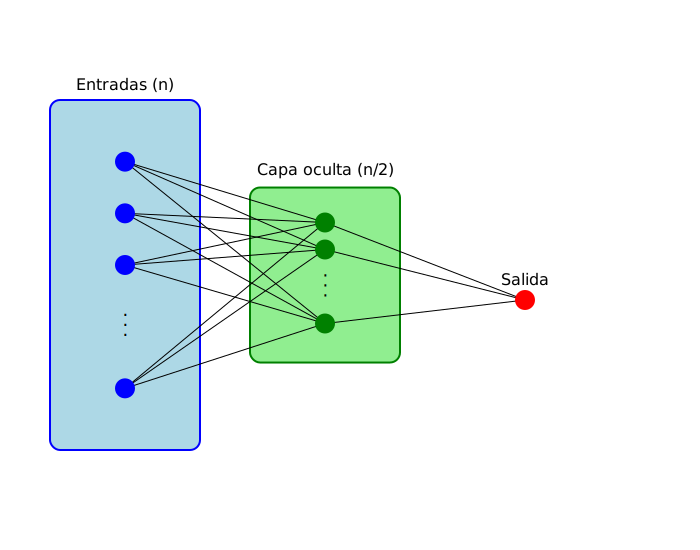
\includegraphics[width=0.8\textwidth]{./img/modelo/arquitecturas/arqnmediosBIN.pdf}
    \caption{Arquitectura del modelo con $n/2$ neuronas en la capa oculta siendo \textit{n} el número de parámetros de entrada.}
    \label{fig:arqnmediosBIN}
\end{figure}

\paragraph{Ventajas (\textit{n/2})}
\begin{itemize}
	\item El riesgo de sobreajuste es menor, esto es especialmente importante si no se utiliza validación cruzada o el conjunto de datos de entrenamiento es pequeño o simple \cite{chollet2017deep}.
	\item  Al tener un número de neuronas menor, tanto la función  de pérdida como el algoritmo de optimización, tardan menos en realizar los cálculos de los ajustes de los pesos y sesgos del modelo. Este menor coste de cálculo se refleja directamente en el tiempo necesario para entrenar el modelo y en el tiempo de respuesta del mismo una vez entrenado \cite{goodfellow2016deep}.
	\item Un número bajo de neuronas es especialmente útil cuando los datos son linealmente separables o poco complejos \cite{ruck1996hidden}.
\end{itemize}
\paragraph{Inconvenientes (\textit{n/2})}
\begin{itemize}
	\item Si las relaciones entre los datos son demasiado complejas, el moelo puede sufrir \textit{underfitting} o subajuste \cite{goodfellow2016deep}.
	\item Sensibilidad alta a la inicialización de los pesos, lo que puede provocar que un porcentaje alto de neuronas no se utilicen por tener pesos iguales o muy cercanos a 0. Esto implica que parte de la capacidad de la red quede inutilizada, empeorando el rendimiento incluso en problemas simples \cite{glorot2010understanding}.
\end{itemize}

Tras comentar cuales son las principales ventajas e inconvenientes de utilizar una capa oculta con un número de neuronas igual a la mitad de los atributos del modelo, aparentemente, las propiedades del conjunto de datos que se utiliza para entrenar al modelo no son las idóneas para esta arquitectura y no se esperan resultados especialmente destacables.

\subsection{Capa oculta con el mismo número de neuronas que atributos de entrada}\label{sec:VIBIN49}
En este apartado se comentan cuales son las principales ventajas e inconvenientes, a priori, de un modelo de clasificación binaria con un número de neuronas en la capa oculta igual al número de parámetros que recibe el modelo, como la que se muestra en la Figura \ref{fig:arqnBIN}.

\begin{figure}[H]
    \centering
    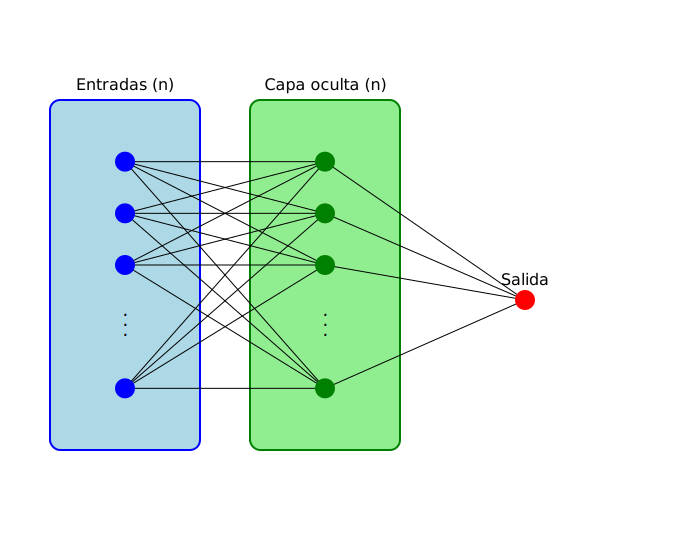
\includegraphics[width=0.8\textwidth]{./img/modelo/arquitecturas/arqnBIN.pdf}
    \caption{Arquitectura del modelo con \textit{n} neuronas en la capa oculta siendo \textit{n} el número de parámetros de entrada.}
    \label{fig:arqnBIN}
\end{figure}

\paragraph{Ventajas (\textit{n})}
\begin{itemize}
	\item La capacidad y la generalización están balanceadas, esto significa que el modelo evita tanto el sobreajuste como el subajuste \cite{zhang2016understanding}.
	\item Es capaz de modelar relaciones más complejas entre conjuntos de datos que arquitecturas con un número de neuronas menor, lo que es especialmente útil en problemas con relaciones no lineales entre sus datos \cite{goodfellow2016deep}.
	\item Son computacionalmente más eficientes que arquitecturas con un número elevado de neuronas en la capa oculta \cite{bengio2006greedy}. 
\end{itemize}
\paragraph{Inconvenientes(\textit{n})}
\begin{itemize}
	\item Puede resultar insuficiente en problemas demasiado complejos o con un gran volumen de datos \cite{hochreiter1997long}.
	\item Si el conjunto de datos utilizado para entrenar el modelo es pequeño puede sobreajustar \cite{yamada2018understanding}.
\end{itemize}

Tras comentar cuales son las principales ventajas e inconvenientes de utilizar una capa oculta con el mismo número de neuronas que entradas recibe el modelo, aparentemente, esta arquitectura ofrecerá resultados significativamente positivos gracias a su equilibrio y balanceo.

\subsection{Capa oculta con el doble de neuronas que atributos de entrada}\label{sec:VIBIN98}
En este apartado se comentan cuales son las principales ventajas e inconvenientes, a priori, de un modelo de clasificación binaria con el doble de neuronas en la capa oculta que parámetros recibe el modelo, como la que se muestra en la Figura \ref{fig:arqnnBIN}.

\begin{figure}[H]
    \centering
    \includegraphics[width=0.8\textwidth]{./img/modelo/arquitecturas/arqnnBIN.pdf}
    \caption{Arquitectura del modelo con $2n$ neuronas en la capa oculta siendo \textit{n} el número de parámetros de entrada.}
    \label{fig:arqnnBIN}
\end{figure}

\paragraph{Ventajas (2n)}
\begin{itemize}
	\item Alta capacidad de aprendizaje, lo que se traduce como la posibilidad de capturar patrones de datos muy complejos que no son lineales ni perceptibles en un análisis superficial del problema \cite{goodfellow2016deep}.
	\item Cuanto mayor es el conjunto de datos mejor se ajustan los pesos \cite{sun2017survey}.
	\item Es menos propenso a subajustar que otras arquitecutras \cite{bishop2006pattern}.
\end{itemize}
\paragraph{Inconvenientes (2n)}
\begin{itemize}
	\item El riesgo de sobreajuste es elevado, memorizando de esta manera ruido en vez de aprender los patrones generalizables \cite{bishop2006pattern}.
	\item Nivel computacional más elevado, lo que se refleja en el tiempo necesario de entrenamiento de esta arquitectura y en su posterior tiempo de respuesta \cite{goodfellow2016deep}.
	\item Si el número de muestras del conjunto de datos es bajo tiende a sobreajustar \cite{overfitting2008}.
\end{itemize}

Tras comentar cuales son las principales ventajas e inconvenientes de utilizar una capa oculta con un número de neuronas igual al doble de los parámetros del modelo, aparentemente, esta arquitectura obtendrá mejores resultados si los parámetros no tiene relaciones lineales. En cambio, si los datos presentan relaciones lineales tiene más probabilidades de sobreajustar los pesos del modelo, lo que implicaría que le modelo no ha sido capaz de converger a una solución genérica.




\section{Estructura/Arquitecturas de los modelos de clasificación multiclase desarrollados}
En esta sección se abordan cuales son las arquitecturas a desarrollar para el modelo de clasificación multiclase. Como se comenta en la Sección \ref{sec:disMUL} \nameref{sec:disMUL}, la diferencia entre las arquitecturas radica en el tamaño de la capa oculta del modelo.

Para el desarrollo de las diferentes arquitecturas, se ha optado por realizar experimentos de entrenamiento del modelo de clasificación multiclase con un tamaño de ventana oculta igual a:

\begin{itemize}

	\item \textbf{MCM25}: La mitad del número de atributos que recibe el modelo
	\item \textbf{MCM49}: El mismo número que atributos que tiene el modelo.
	\item \textbf{MCM98}: El doble del número de atributos. 

\end{itemize}

Esto equivale a un tamaño de la capa de venta oculta de 25, 49 y 98 respectivamente, de forma análoga a como sucede con las arquitecturas del modelo de clasificación binaria.

A continuación, se comentan las posibles ventajas e inconvenientes de cada arquitectura que se esperan antes de realizar los experimentos.

\subsection{Capa oculta con la mitad de neuronas que atributos de entrada}\label{sec:VIMUL25}
En este apartado se comentan cuales son las principales ventajas e inconvenientes, a priori, de un modelo de clasificación multiclase con un número de neuronas en la capa oculta igual a la mitad del número de parámetros que recibe el modelo, como la que se muestra en la Figura \ref{fig:arqnmediosMUL}.

\begin{figure}[H]
    \centering
    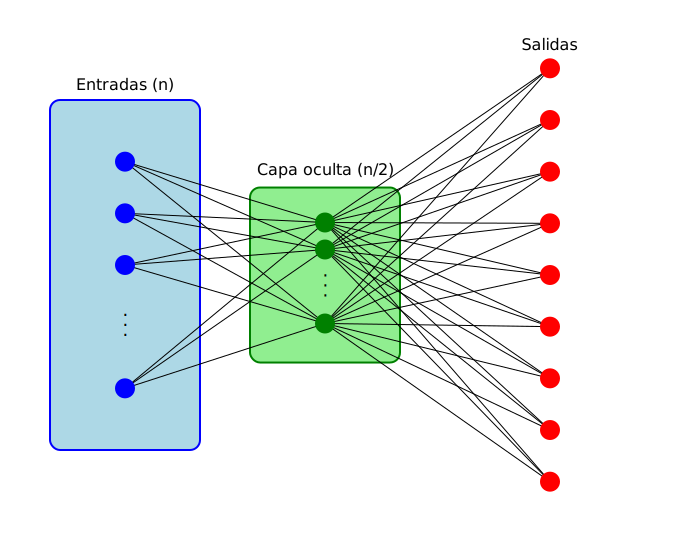
\includegraphics[width=0.8\textwidth]{./img/modelo/arquitecturas/arqnmediosMUL.pdf}
    \caption{Arquitectura del modelo con n/2 neuronas en la capa oculta siendo n el número de parámetros de entrada.}
    \label{fig:arqnmediosMUL}
\end{figure}

\paragraph{Ventajas (n/2)}
\begin{itemize}
	\item Un número reducido de neuronas en la capa oculta limita la capacidad del modelo para memorizar patrones dominantes, lo cual puede ayudar a mitigar el sobreajuste hacia las clases mayoritarias del conjunto de entrenamiento \cite{zhang2016understanding}.
	\item Al reducirse la complejidad del modelo, se disminuye el tiempo necesario para calcular los gradientes durante el entrenamiento y, en consecuencia, también el tiempo de respuesta durante la inferencia \cite{han2015learning}.
	\item En presencia de clases desbalanceadas, un modelo menos expresivo puede favorecer una mayor estabilidad en el aprendizaje, evitando que la red se especialice únicamente en las clases más frecuentes \cite{he2009learning}.

\end{itemize}
\paragraph{Inconvenientes (n/2)}
\begin{itemize}
	\item Un número bajo de neuronas puede limitar la capacidad del modelo para aprender representaciones suficientes de las clases minoritarias, especialmente si estas presentan patrones complejos o poco diferenciados \cite{chawla2004editorial}.
	\item La capacidad reducida del modelo puede dificultar la separación entre clases en problemas multiclase, afectando negativamente al rendimiento en métricas sensibles al desbalance como el \textit{macro Recall} o el \textit{macro F1-score} \cite{he2009learning}.
	\item Si el número de parámetros de entrada es muy alto, una capa oculta con solo la mitad de neuronas podría actuar como un cuello de botella, perdiéndose información útil para distinguir correctamente entre clases poco representadas \cite{goodfellow2016deep}.

\end{itemize}

Tras comentar cuales son las principales ventajas e inconvenientes de utilizar una capa oculta con un número de neuronas igual a la mitad de los parámetros del modelo, aparentemente, las propiedades del conjunto de datos que se utiliza para entrenar al modelo no son las idóneas para esta arquitectura y no se esperan resultados especialmente destacables. Debido al alto desbalanceo entre clases, se espera que esta arquitectura proporcione resultados peores que su equivalente del modelo de clasificación binaria.

\subsection{Capa oculta con el mismo número de neuronas que atributos de entrada}\label{sec:VIMUL49}
En este apartado se comentan cuales son las principales ventajas e inconvenientes, a priori, de un modelo de clasificación multiclase con un número de neuronas en la capa oculta igual al número de parámetros que recibe el modelo, como la que se muestra en la Figura \ref{fig:arqnMUL}.

\begin{figure}[H]
    \centering
    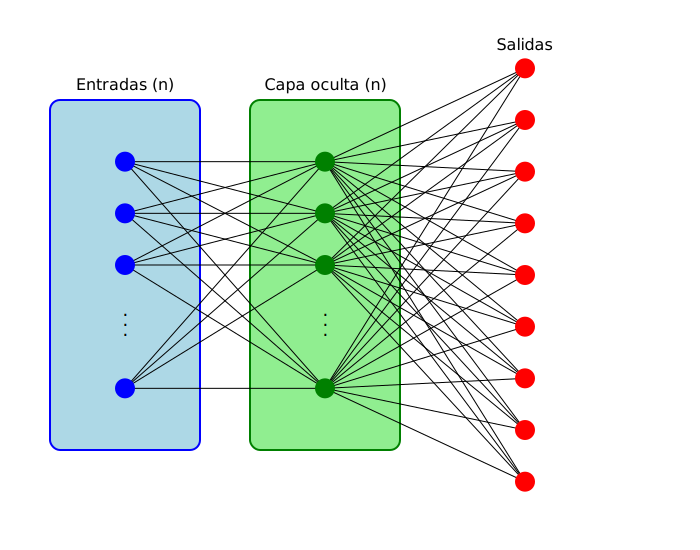
\includegraphics[width=0.8\textwidth]{./img/modelo/arquitecturas/arqnMUL.pdf}
    \caption{Arquitectura del modelo con n neuronas en la capa oculta siendo n el número de parámetros de entrada.}
    \label{fig:arqnMUL}
\end{figure}

\paragraph{Ventajas (n)}
\begin{itemize}
	\item Un número de neuronas igual al de parámetros de entrada proporciona al modelo una capacidad representativa suficiente para capturar patrones relevantes tanto en clases frecuentes como en las minoritarias \cite{heaton2017deep}.
	\item Esta configuración ofrece un equilibrio razonable entre complejidad y eficiencia computacional, manteniendo un coste de entrenamiento y de inferencia moderado sin comprometer la expresividad del modelo \cite{goodfellow2016deep}.
	\item Permite al modelo adaptar sus pesos de manera más flexible, facilitando el aprendizaje de límites de decisión más precisos entre clases desbalanceadas sin riesgo inmediato de sobreajuste \cite{he2009learning}.

\end{itemize}
\paragraph{Inconvenientes (n)}
\begin{itemize}
	\item Aun sin ser excesivo, este tamaño puede generar cierta sobreadaptación a las clases mayoritarias si no se aplican mecanismos de regularización adecuados \cite{goodfellow2016deep}.
	\item En conjuntos de datos muy desbalanceados, esta configuración puede no ser suficiente para compensar la escasa representación de clases minoritarias, especialmente si estas requieren una mayor capacidad para ser correctamente diferenciadas \cite{he2009learning}.
	\item Si las características de entrada tienen una alta correlación entre sí, mantener el mismo número de neuronas puede introducir redundancia, afectando la eficiencia del aprendizaje y aumentando el riesgo de converger a soluciones deficientes \cite{bengio2013representation}.
\end{itemize}

Tras comentar cuales son las principales ventajas e inconvenientes de utilizar una capa oculta con el mismo número de neuronas que parámetros recibe el modelo, aparentemente, esta arquitectura ofrecera resultados significativamente positivos gracias a su equilibrio. Aunque, si las clases que tienen un número inferior de muestras, tienen relaciones complejas entre sus datos, esta arquitectura puede ser insuficiente para obtener un modelo capaz de distinguir entre algunas de las clases más minoritarias.

\subsection{Capa oculta con el doble de neuronas que atributos de entrada}\label{sec:VIMUL98}
En este apartado se comentan cuales son las principales ventajas e inconvenientes, a priori, de un modelo de clasificación multiclase con el doble de neuronas en la capa oculta que parámetros recibe el modelo, como la que se muestra en la Figura \ref{fig:arqnnMUL}.

\begin{figure}[H]
    \centering
    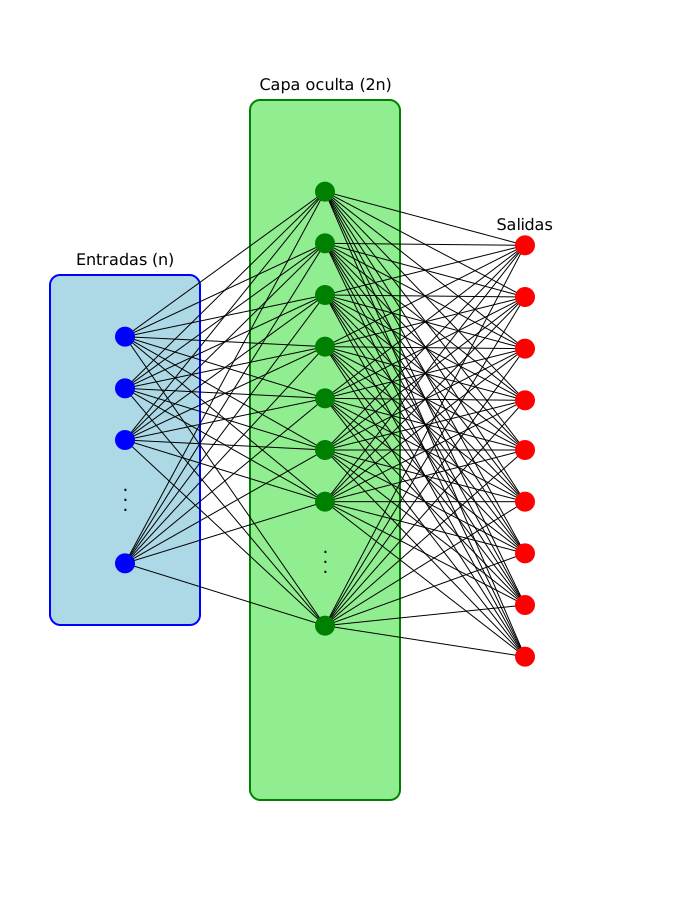
\includegraphics[width=0.8\textwidth]{./img/modelo/arquitecturas/arqnnMUL.pdf}
    \caption{Arquitectura del modelo con 2n neuronas en la capa oculta siendo n el número de parámetros de entrada.}
    \label{fig:arqnnMUL}
\end{figure}

\paragraph{Ventajas (2n)}
\begin{itemize}
	\item Una capa oculta más amplia incrementa la capacidad del modelo para aprender representaciones complejas, lo que puede ser especialmente útil para distinguir correctamente clases minoritarias con patrones sutiles o poco definidos \cite{srivastava2014dropout}.
	\item Esta configuración ofrece una mayor flexibilidad al modelo para aproximar funciones no lineales, favoreciendo una mejor separación entre clases en escenarios multiclase con alta variabilidad entre categorías \cite{bishop2006pattern}.
	\item Al disponer de más neuronas, el modelo tiene mayor margen para explorar combinaciones de características relevantes durante el entrenamiento, lo cual puede traducirse en una mejora de métricas como macro F1 o recall por clase \cite{liu2020deep}.
\end{itemize}

\paragraph{Inconvenientes (2n)}
\begin{itemize}
	\item El aumento en el número de parámetros incrementa el riesgo de sobreajuste, especialmente en presencia de clases mayoritarias dominantes o cuando el conjunto de entrenamiento es reducido \cite{srivastava2014dropout}.
	\item Un modelo con mayor complejidad requiere más recursos computacionales y tiempos de entrenamiento más prolongados, lo que puede dificultar su implementación en entornos con restricciones de capacidad o temporales \cite{han2015deep}.
	\item Si no se utilizan mecanismos de control adecuados (como regularización o balanceo de clases), es posible que el modelo aprenda a ajustar principalmente las clases frecuentes, sin mejorar sustancialmente el rendimiento en las minoritarias \cite{chawla2002smote}.

\end{itemize}

Tras comentar cuales son las principales ventajas e inconvenientes de utilizar una capa oculta con un número de neuronas igual al doble de los parámetros del modelo, aparentemente, esta arqutectura será la que mejores resultados obtenga en la detección de clases minoritarias al tener la capacidad de aprender representaciones más complejas. Sin embargo, esta arquitectura es más propensa a sobreajustes debido la presencia de las clases mayoritarias.

\subsection{Diseños del modelo de clasificación multiclase descartados} \label{subsec:MCMdescart}

Debido a la complejidad del problema al resolver, se probaron otros diseños diferentes a los finalmente utilizados que fueron descartados por no obtner los resultados esperados. A continuación, se detalla cuales fueron estos diseños descartados, la motivación que llevo a probarlo y cuales fueron sus resultados.

Durante las pruebas realizadas antes de ejecutar los experimentos para encontrar la combinación de hiperparámetros que mejor convergían para este modelo, se detectó que el desbalanceo de las clases afectaba de manera significativa a los resultados que se obtenían. Con el objetivo de reducir el impacto del desbalanceo en el entrenamiento del modelo, se optó por ejecutar experimentos para sondear el desempeño de diferentes técnicas. Los resultados de estos experimentos se muestran en la Figura  \ref{fig:MULpruebas}, junto con los resultados que obtuvieron estas combinaciones de técnicas en la métrica \textit{F1 weighted}.


\begin{figure}[H]
    \centering
    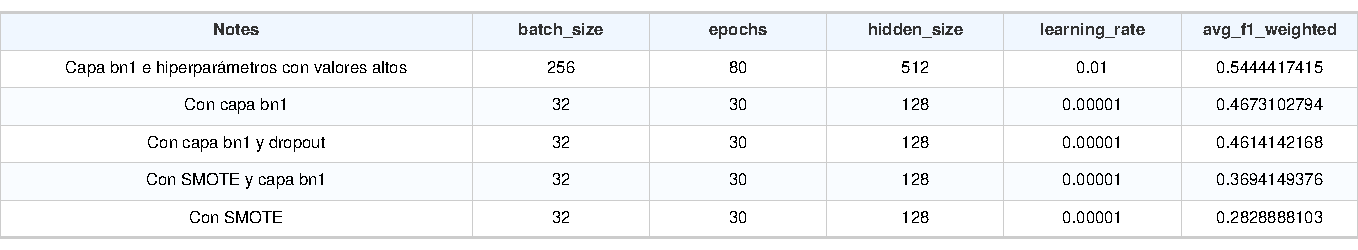
\includegraphics[width=0.95\textwidth]{./img/modelo/resultados/MULPRUEBAS.pdf}
    \caption{Resultados de los diferentes diseños probados para el modelo de clasifcación multiclase.}
    \label{fig:MULpruebas}
\end{figure}

Sin embargo, tras realizar una serie de pruebas, el modelo diseñado que implementaba  \texttt{SMOTE} fue el que peores resultados dió. Por eso motivo, se combinó con la función \texttt{Batch Normalization} explicada en la Sección \ref{subsubsection:bn} \nameref{subsubsection:bn}.

Los resultados de \texttt{Batch Normalization} (bn1) y \texttt{SMOTE} mostrados en la Figura \ref{fig:MULpruebas} fueron algo mejores que los valores obtenidos de las pruebas realizadas solo con \texttt{SMOTE}. Como se noto una mejora en el desempeño del modelo al utilizar bn1, pero los resultados obtenidos seguían sin ser los esperados, se probó con combinaciones de diseño utilizando bn1 con otras técnicas.

Con la implementación del \texttt{Dropout}, los resultados mejoraron significativamente. Sin embargo, el diseño del modelo que solo utilizaba bn1 obtuvo mejores resultados de media que aquel que utilizaba bn1 y \textit{dropout}. Por este motivo, el diseño utilizado en los experimentos solo implementa \texttt{Batch Normalization}. Además, tras realizar pruebas con valores altos para los hiperparámetros, se obtuvieron unos resultados con una convergencia mayor que la de las pruebas realizadas con valores menores, tal y como puede observarse en la Figura \ref{fig:MULpruebas}, lo que incentivó a aumentar los valores de los hiperparámetros probados, tal y como se puede observar en la sección anterior.




\section{Implementación del modelo neuronal de clasificación binaria} \label{sec.modBIN}
En esta sección se describe tanto el proposito como los procedimientos empleados para el desarrollo del modelo de clasificación binaria. Se detalla el proceso de selección de hiperparámetros, así como las distintas arquitecturas diseñadas con el fin de identificar la combinación que optimiza el rendimiento del modelo. Además, se presenta una comparación entre las arquitecturas evaluadas para determinar la más adecuada.

%Finalmente, se especifican las métricas utilizadas para la evaluación y selección de las mejores combinaciones de hiperparámetros.

\subsection{Proposito del modelo de clasificación binaria}
El modelo de clasificación binaria se ha diseñado con el objetivo de identificar de manera precisa y eficiente, si una instancia de tráfico de red corresponde a una actividad legítima o a un comportamiento malicioso. Su función principal consiste en distinguir entre accesos normales y posibles intentos de intrusión, permitiendo así la detección temprana de ataques y contribuyendo a la protección proactiva de los sistemas informáticos.

\subsection{Diseño del modelo e hiperparámetros seleccionados} \label{sec:disBIN}
Para diseñar la arquitectura del modelo, se ha desarrollado la clase Modelo. Esta clase está conformada por dos métodos, la primera corresponde con la inicialización de la clase, y la segunda con la arquitectura utilizada para este modelo.

Como se puede observar en la Figura \ref{fig:modBIN}, el modelo está compuesto por dos capas. La \texttt{capa1} tiene un número de entradas igual al número de parámetros que posee el \textit{dataset}, como se comenta en la Sección \ref{sec.prep-datos}, el número de entradas del modelo es 49. El número de salidas depende del parámetro \textit{ventaOculta}, con el que se llama a la función de inicialización del modelo. El número de salidas de la \texttt{capa1} será precisamente el que determine la arquitectura específica que se utiliza. Por su parte, la \texttt{capa2} recibe como entrada el número de salidas de la \texttt{capa1} y al tratarse de la capa final de un modelo de clasificación binaria, esta capa tendrá una única salida.

Debido a que la función de pérdida utilizada para entrenar el modelo es \texttt{BCEWithLogitsLoss()}, que ya aplica la función sigmoidea, sería contraproducente aplicar la función sigmoidea sobre la salida del modelo para su entrenamiento.

\begin{figure}[H]
    \centering
    \includegraphics[width=0.8\textwidth]{./img/modelo/codigo/modeloBIN.png}
    \caption{Definición de la clase del modelo de clasificación binaria.}
    \label{fig:modBIN}
\end{figure}

Como algoritmo de optimización para el entrenamiento del modelo de clasificación binaria, se ha optado por utilizar \texttt{AdamW()}. Como se comenta en la sección \ref{sec:alg-opt} \nameref{sec:alg-opt}, se ha demostrado que AdamW es más eficaz en la prevención de sobreajuste en redes neuronales que otros algoritmos de optimización. Además, permite una mejor generalización en problemas con grandes volúmenes de datos como el que se trata en este proyecto.

Los hiperparámetros que han sido seleccionados para encontrar la mejor configuración para el modelo de clasificación binaria diseñado son: el batch size, la tasa de aprendizaje (learning rate) y el número de épocas. Estos hiperparámetros resultan imprescindibles en el entrenamiento de modelos de clasificación binaria, dado que influyen directamente en la eficiencia del proceso de optimización y en la calidad del modelo resultante.

Como se comenta en la sección \ref{sec:paramhiper} \nameref{sec:paramhiper}, los hiperparámetros controlan el comportamiento del proceso de entrenamiento y afectan la capacidad del modelo para aprender patrones complejos de los datos. Teniendo en cuenta las características de cada hiperparámetro, se han escogido los siguientes valores para los experimentos del entrenamiento del modelo binario con el objetivo de encontrar la mejor combinación de ellos.

\begin{itemize}
	\item \textbf{\textit{Batch size}}: Teniendo en cuenta el tamaño de los datos que se utilizan para la fase de entrenamiento del modelo binario, se han considerado que los valores que se muestran en la Tabla \ref{tab:hiperBIN}, eran apropiados y suficientemente dispares como para notar diferencias significativas en los resultados de la ejecución de los experimentos.
	\item \textbf{\textit{Learning rate}}: Siguiendo los avisos de la sección anterior en la que se explicaba el propósito y características de cada hiperparámetro, se ha optado por elegir unos valores con los que se espera que el modelo converja sin sobreajustarse ni se exceda en el tiempo de obtención de una solución válida.
	\item \textbf{Épocas}: De forma similar a como sucede con la tase de aprendizaje, un valor excesivamente bajo en el número de épocas puede provocar que el modelo no converja. Sin embargo, un número demasiado alto de épocas provoca sobreajuste en el modelo.
\end{itemize}

\begin{table}[H]
\centering
\begin{tabular}{|c|c|}
\hline
\textbf{Hiperparámetro} & \textbf{Posibles valores} \\ \hline
\textit{Batch size} & [2000, 10000, 15000, 20000] \\ \hline
\textit{Learning rate} & [0.01, 0.001, 0.0001] \\ \hline
Épocas & [10, 20, 30] \\ \hline
\end{tabular}
\caption{Valores de los hiperparámetros utilizados en los experimentos del modelo de clasificación binaria.}
\label{tab:hiperBIN}
\end{table}

Una vez definidos los valores de los hiperparámetros con los que se probaran durante la búsqueda de la mejor configuración, se divide el conjunto de entrenamiento en los correspondientes \textit{folds} que se utilizan en la validación cruzada, dentro del bucle que prueba con todas las configuraciones de hiperparámetros. Después, se inicializa \texttt{wandb} para registrar los resultados de cada experimento. A continuación, se crean los objetos de clase \texttt{DatasetTFG} que utilizaran los correspondiente \texttt{DataLoaders}  durante el entrenamiento y la validación de los modelos. En la Figura \ref{fig:DatasetTFG} se muestra el código utilizado para describir la clase \texttt{DatasetTFG}. 


\begin{figure}[H]
    \centering
    \includegraphics[width=0.8\textwidth]{./img/modelo/codigo/DatasetTFG.png}
    \caption{Definición de la clase \texttt{DatasetTFG}.}
    \label{fig:DatasetTFG}
\end{figure}

Una vez inicializados todos los objetos necesarios se entrena al modelo dentro del bucle de entrenamiento cuyo número de iteraciones depende del hiperparámetros \textit{Epochs}, tal y como se puede observar en la Figura \ref{fig:EntrenamientoCVBIN}. Para comprobar los resultados del entrenamiento del modelo, se ejecuta el bucle de validación del modelo entrenado para obtener las métricas que se almacenan en la herramienta \texttt{wandb}.



\begin{figure}[H]
    \centering
    \includegraphics[width=0.8\textwidth]{./img/modelo/codigo/EntrenamientoCVBIN.png}
    \caption{Bucle de entrenamiento del modelo de clasificación binaria.}
    \label{fig:EntrenamientoCVBIN}
\end{figure}



\section{Implementación del modelo neuronal de clasificación multiclase}
Esta sección aborda los objetivos y procedimientos aplicados en el desarrollo del modelo de clasificación multiclase. Se describe el proceso llevado a cabo para la selección de hiperparámetros, con el propósito de identificar la configuración que maximiza el desempeño del modelo.

\subsection{Proposito del modelo de clasificación multiclase}

El modelo de clasificación multiclase se ha diseñado con el objetivo de identificar de manera precisa y eficiente, a que tipo de ataque corresponde una conexión maliciosa que el modelo de clasificación binaria ha clasificado previamente como intrusiva. Su función principal consiste en distinguir entre 9 clases diferentes de ataques que se detallan en la sección \ref{sec.tipo-ataques} \nameref{sec.tipo-ataques}, contribuyendo a la protección proactiva de los sistemas informáticos.

\subsection{Diseño del modelo e hiperparámetros seleccionados} \label{sec:disMUL}
Para diseñar la arquitectura del modelo, se ha desarrollado la clase \texttt{ModeloMulticlase}. Esta clase está conformada por dos métodos, la primera corresponde con la inicialización de la clase, y la segunda con la arquitectura utilizada para este modelo.

Como se puede observar en la Figura \ref{fig:modMUL}, el modelo está compuesto por dos capas. La capa1 tiene un número de entradas igual al número de atributos que poseen los datos utilizados para entrenar al modelo y un número de salidas que depende del parámetro \textit{ventaOculta}, con el que se llama a la función de inicialización del modelo. El número de salidas de la capa1 será precisamente el que determine la arquitectura específica que se utiliza. Una vez que los datos pasan por la \texttt{capa1}, se utiliza la técnica \texttt{Batch Normalization}. 

Como se explica anteriormente, las redes neuronales necesitan funciones no lineales para aprender relaciones complejas entre las entradas y salidas, por este motivo, se aplica la función de activación ReLU depués del \textit{Batch Normalization}. Sin activaciones como ReLU, toda la red sería equivalente a una simple transformación lineal, sin capacidad de aprendizaje automático. Que el modelo presente una alta capacidad de aprendizaje automático es esencial para los modelos de clasifiación multiclase cuya complejidad es mucho mayor que la de los modelos de clasificación binaria.

Para finalizar, la \texttt{capa2} recibe como entrada las salidas de la \texttt{capa1} y al tratarse de la capa final de un modelo de clasificación multiclase, esta capa tendrá una salida por cada clase que es capaz de identificar el modelo.

Por lo general, en clasificación multiclase, la salida del modelo suele ser un vector de \textit{logits} (valores sin escalar), uno por cada clase. La función de activación Softmax transforma esos \textit{logits} en probabilidades, es decir, cada valor representa lo probable que es que los datos que han entrado al modelo, pertenezca a esa clase. Debido a que durante el entrenamiento, se utiliza el \textit{frameworks} PyTorch, no es necesario aplicar Softmax a la salida del modelo cuando se utiliza la función de pérdida \texttt{CrossEntropyLoss}. La razón es que función \texttt{CrossEntropyLoss}, ya incluye \texttt{Softmax} internamente por razones de eficiencia y estabilidad numérica.

\begin{figure}[H]
    \centering
    \includegraphics[width=0.8\textwidth]{./img/modelo/codigo/modeloMUL.png}
    \caption{Estructura del modelo de clasificación multiclase diseñada.}
    \label{fig:modMUL}
\end{figure}

Al igual que en el caso de la calsificación binaria para evitar el sobreajuste del modelo y obtener valores de las predicciones más confiables que se utilizarán para la evaluación del rendimiento del modelo, se utiliza validación cruzada \texttt{k-fold}. Como se explica en la sección anterior, la validación cruzada consiste en dividir los datos de entrenamiento en n \textit{folds} que se utilizan para entrenar al modelo con $n-1$ \textit{folds} y después validar el modelo entrenado con el fold que no se ha utilizado para entrenarlo. Este proceso se repite para los n \textit{folds} y en cada iteración es un \textit{fold} distinto el que no se utiliza para el entrenamiento. Una vez completadas las iteraciones se extraen las medias de las métricas obtenidas con cada \textit{fold} durante la validación. Para entrenar el modelo de clasificación multiclase, se ha utilizado StratifiedKFold() que como su nombre indica, estratifica los \textit{folds} para que las proporciones de las clases de los datos utilizados para el entrenamiento se mantengan similares en cada \textit{fold} y no se creen \textit{folds} con un único tipo de clase. Estratificar los datos es especialmente crítico para aquellos datasets cuyos datos están muy desbalanceados como es el caso de los datos utilizados para entrenar los modelos de este proyecto. Concretamente, tras el tratamiento de los datos, existen 284 veces más muestras de la clase con mayor presencia en el \textit{dataset}, que de la clase con menor presencias. Para el entrenamiento del modelo de clasificación multiclase, se ha optado por utilizar validación cruzada \texttt{StratifiedKFold} con 5 \textit{folds} o divisiones.

Como algoritmo de optimización para el entrenamiento del modelo de clasificación multiclase, se ha optado por utilizar AdamW(). Como se comenta en la sección \ref{sec:alg-opt} \nameref{sec:alg-opt}, se ha demostrado que AdamW es más eficaz en la prevención de sobreajuste en redes neuronales que otros algoritmos de optimización.

Los hiperparámetros que han sido seleccionados para encontrar la mejor configuración para el modelo de clasificación multiclase diseñado son: el \textit{batch size}, la tasa de aprendizaje (\textit{learning rate}) y el número de épocas. Estos hiperparámetros resultan imprescindibles en el entrenamiento de modelos de clasificación multiclase, dado que influyen directamente en la eficiencia del proceso de optimización y en la calidad del modelo resultante.

Como se comenta en la sección \ref{sec:paramhiper} \nameref{sec:paramhiper}, los hiperparámetros controlan el comportamiento del proceso de entrenamiento y afectan la capacidad del modelo para aprender patrones complejos de los datos. Teniendo en cuenta las características de cada hiperparámetro, se han escogido los siguientes valores para los experimentos del entrenamiento del modelo multiclase con el objetivo de encontrar la mejor combinación de ellos.

\begin{itemize}
	\item \textbf{\textit{Batch size}}: Teniendo en cuenta el tamaño de los datos que se utilizan para la fase de entrenamiento del modelo de clasificación multiclase, se han considerado que los valores que se muestan en la Tabla \ref{tab:hiperMUL}, eran apropiados y suficientemente dispares como para notar diferencias significativas en los resultados de la ejecución de los experimentos.
	\item \textbf{\textit{Learning rate}}: Siguiendo los avisos de la sección anterior en la que se explicaba el propósito y características de cada hiperparámetro, se ha optado por elegir unos valores con los que se espera que el modelo converja sin sobreajustarse ni se exceda en el tiempo de obtención de una solución válida.
	\item \textbf{Épocas}: De forma similar a como sucede con la tase de aprendizaje, un valor excesivamente bajo en el número de épocas puede provocar que el modelo no converja. Sin embargo, un número demasiado alto de épocas provoca sobreajuste en el modelo.
\end{itemize}

\begin{table}[H]
\centering
\begin{tabular}{|c|c|}
\hline
\textbf{Hiperparámetro} & \textbf{Posibles valores} \\ \hline
\textit{Batch size} & [32, 64, 128, 256, 512] \\ \hline
\textit{Learning rate} & [$1e-2$, $1e-3$, $1e-4$, $1e-5$] \\ \hline
Épocas & [30, 50, 80, 100] \\ \hline
\end{tabular}
\caption{Valores de los hiperparámetros utilizados en los experimentos del modelo de clasificación multiclase.}
\label{tab:hiperMUL}
\end{table}


Una vez definidos los valores de los hiperparámetros que se evaluarán durante el proceso de búsqueda de la mejor configuración, se procede a dividir el conjunto de entrenamiento en los correspondientes \textit{folds}, los cuales se emplean en la validación cruzada dentro del ciclo que recorre todas las combinaciones posibles de hiperparámetros. Posteriormente, se inicializa la herramienta \texttt{wandb} con el fin de registrar automáticamente los resultados de cada experimento ejecutado. A continuación, se instancian los objetos de la clase \texttt{DatasetTFG}, que serán utilizados por los respectivos \texttt{DataLoaders} tanto en la fase de entrenamiento como en la de validación del modelo multiclase. 

Una vez inicializados todos los componentes necesarios, se procede al entrenamiento del modelo dentro del ciclo correspondiente, cuyo número de iteraciones está determinado por el hiperparámetro \textit{Epochs}. Para obtener las métricas que se almacenaran en la herramienta \texttt{wandb}, finalmente se ejecuta el bucle de validación con el \textit{fold} correspondiente tal y como se muestra en la Figura  \ref{fig:ValidacionCVMUL}.

\begin{figure}[H]
    \centering
    \includegraphics[width=0.8\textwidth]{./img/modelo/codigo/ValidacionCVMUL.png}
    \caption{Bucle de validación del modelo de clasificación multiclase.}
    \label{fig:ValidacionCVMUL}
\end{figure}



La convergencia de los modelos de clasifcación multiclase es mucho más complicada que en los modelos de clasificación binaria. Esto se debe a que en los modelos de clasificación binaria hay 4 posibles respuestas (VP, VN, FP, FN), mientras que en el  modelo de clasificación multiclase que se propone en este proyecto hay 9 clases por 9 posibilidades de respuesta por clase, lo que suma un total de 81 posibles respuestas. Para encontrar una configuración de los hiperparámetros que se ajuste mejor a la complejidad de este problema, se han probado más combinaciones de valores de los hiperparámetros en el modelo de clasificación multiclase que en el modelo de clasificación binaria. El aumento del número de experimentos se ha realizado teniendo en cuenta que el número de muestras de conexiones maliciosas es mucho menor que el número total de conexiones que se ha utilizado para entrenar el modelo de clasifcación binaria. Esto se traduce en que el tiempo de ejecución de los experimentos de ambos modelos ha sido similar compensando el número de muestras con el número de experimentos.




\section{Selección de modelos de clasificación binaria}
En esta sección se pueden observar los resultados de los experimentos realizados con los posibles valores de los hiperparámetros comentados en la sección \ref{sec:disBIN} \nameref{sec:disBIN}.

La plataforma \textit{Weights \& Biases} (wandb) se emplea para el seguimiento de experimentos, registro de hiperparámetros, métricas y artefactos de los modelos desarrollados en este trabajo. Esta herramienta ofrece una interfaz visual e interconectada que permite comparar ejecuciones de entrenamiento en proyectos de clasificación binaria y multiclase. También permite iniciar ejecuciones, almacenar la configuración del experimento, registrar métricas como \textit{Recall} y \textit{F1-weighted}. Además, permite gestionar versiones del modelo y datasets desde su \texttt{API}, lo cual mejora la transparencia, reproducibilidad y eficiencia en el desarrollo de sistemas de detección de conexiones malintencionadas \cite{wandb_tracking}.

\texttt{Wandb} se diseñó con el objetivo de ser la pizarra digital del patrón pirzarra. El patrón arquitectónico pizarra (\textit{blackboard}) se basa en un espacio de trabajo compartido que es accesible por componentes especializados o agentes, los cuales escriben y leen información de forma coordinada y colaborativa. Este enfoque es ideal para integrar etapas de preprocesamiento, inferencia y monitorización, donde cada módulo contribuye con su aporte al cruce de datos y resultados sin acoplamientos rígidos, favoreciendo la modularidad y la adaptabilidad ante cambios en el flujo de trabajo \cite{blackboard_architecture}.

Para medir la eficiencia y eficacia del modelo, se han obtenido las métricas derivadas de la matriz de confusión comentadas en la sección \ref{sec.metricas-bin} \nameref{sec.metricas-bin}. El objetivo del modelo es detectar intrusiones en redes informáticas, por este motivo, los falsos negativos, es decir cuando se produce un ataque o intrusión y no se detecta, pueden tener consecuencias muy catastróficas para el sistema. Teniendo esto en cuenta, la métrica más importante es \textit{Recall}, puesto que es la que se ve más afectada por la presencia de falsos negativos y por este motivo será la que se utilice para crear los \textit{rankings} de esta sección .

Otras métricas relevantes que se muestran en las siguientes figuras son:
\begin{itemize}
	\item \textbf{F1 score}%: Equilibra entre precisión y \textit{recall}. Ideal cuando se necesita rendimiento general en un contexto con mucho desbalanceo como el que se propone en este proyecto.
	\item \textbf{Precisión}%: Si es bajo implica que el modelo detectará muchos falsos positivos, lo que saturaria a los administradores de falsas alarmas y provocaría desconfianza en el modelo.
	\item \textbf{ROC AUC}%: Compara el rendimiento global del modelo, independientemente del umbral. Es especialmente útil para afinar la sensibilidad o \textit{recall}.
\end{itemize}

En las siguientes figuras se hace referencia a los posibles combinaciones de la matriz de confusión en inglés, es decir:
\begin{itemize}
	\item \textbf{tp}: Verdaderos positivos (VP), intrusiones que se han clasificado como intrusiones.
	\item \textbf{tn}: Verdaderos negativos (VN), conexiónes legítimas identificadas como tal.
	\item \textbf{fp}: Falsos positivos (FP), conexiones legítimas clasificadas como intrusiones.
	\item \textbf{fn}: Falsos negativos (FN), intrusiones que se han clasificado como conexiones legítimas.
\end{itemize}

En la Figura \ref{fig:BINhs25}, se encuentran representadas las cinco mejores configuraciones de hiperparámetros para el modelo de clasificación binária con una arquitectura de 25 neuronas (n/2) en la capa oculta. Los resultados obtenidos superan lo esperado tras el análisis de la sección \ref{sec:VIBIN25} para esta arquitectura. La mejor configuración para la arquitectura con la mitad de neuronas en la capa oculta que de parámetros de entrada tiene el modelo, ha sido:
\begin{itemize}
	\item \textbf{\textit{Batch size}}: 15\,000
	\item \textbf{\textit{Epochs}}: 10
	\item \textbf{\textit{Learning rate}}: 0.01
\end{itemize}

\begin{figure}[H]
    \centering
    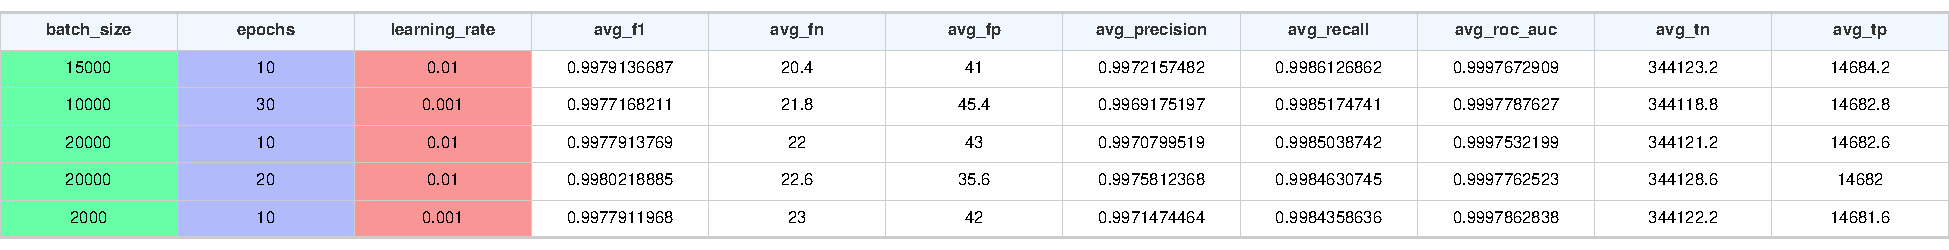
\includegraphics[width=1\textwidth]{./img/modelo/resultados/BINhs25.pdf}
    \caption{Mejores cinco configuraciones de hiperparámetros del modelo de clasificación binaria con una capa oculta de 25 neuronas ($n/2$).}
    \label{fig:BINhs25}
\end{figure}

La matriz de confusión de la mejor configuración de hiperparámetros obtenida en el Modelo de Clasificación Binaria de 25 neuronas (MCB25), es la que se muestra en la Figura \ref{fig:MC_ENT_MCB25}.

\begin{figure}[H]
    \centering
    \includegraphics[width=0.5\textwidth]{./img/modelo/matrices_confusion/MC_ENT_MCB25.png}
    \caption{Matriz de confusión de la mejor configuración de hiperparámetros obtenida en el MCB25 durante la fase de búsqueda.}
    \label{fig:MC_ENT_MCB25}
\end{figure}




La Figura \ref{fig:BINhs49}, muestra la representación de las cinco mejores configuraciones de hiperparámetros para el modelo de clasificación binária con una arquitectura de 49 neuronas (n) en la capa oculta. Los resultados medios obtenidos concuerdan con lo comentado en el análisis de la sección \ref{sec:VIBIN49} para esta arquitectura. La mejor configuración para la arquitectura con la el mismo número de neuronas en la capa oculta que de parámetros de entrada tiene el modelo, ha sido:
\begin{itemize}
	\item \textbf{\textit{Batch size}}: 20\,000
	\item \textbf{\textit{Epochs}}: 10
	\item \textbf{\textit{Learning rate}}: 0.01
\end{itemize}

\begin{figure}[H]
    \centering
    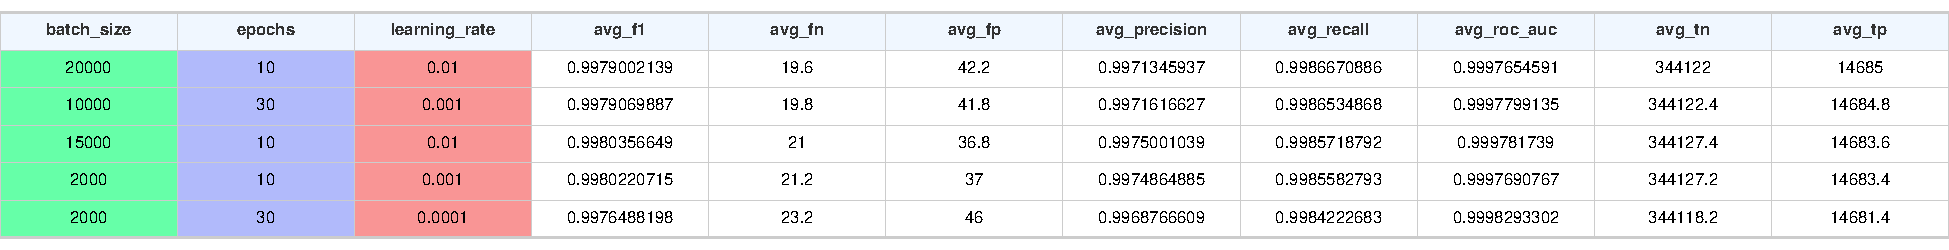
\includegraphics[width=1\textwidth]{./img/modelo/resultados/BINhs49.pdf}
    \caption{Mejores cinco configuraciones de hiperparámetros del modelo de clasificación binaria con una capa oculta de 49 neuronas ($n$).}
    \label{fig:BINhs49}
\end{figure}

La matriz de confusión de la mejor configuración de hiperparámetros obtenida en el Modelo de Clasificación Binaria de 49 neuronas (MCB49), es la que se muestra en la Figura \ref{fig:MC_ENT_MCB49}.

\begin{figure}[H]
    \centering
    \includegraphics[width=0.5\textwidth]{./img/modelo/matrices_confusion/MC_ENT_MCB49.png}
    \caption{Matriz de confusión de la mejor configuración de hiperparámetros obtenida en el MCB49 durante la fase de búsqueda.}
    \label{fig:MC_ENT_MCB49}
\end{figure}


En la Figura \ref{fig:BINhs98}, se encuentran representadas las cinco mejores configuraciones de hiperparámetros para el modelo de clasificación binária con una arquitectura de 98 neuronas (2n) en la capa oculta. Los resultados obtenidos coindiden con lo esperado tras el análisis de la sección \ref{sec:VIBIN98} para esta arquitectura. La mejor configuración para la arquitectura con el doble de neuronas en la capa oculta que de parámetros de entrada tiene el modelo, ha sido:
\begin{itemize}
	\item \textbf{\textit{Batch size}}: 20\,000
	\item \textbf{\textit{Epochs}}: 10
	\item \textbf{\textit{Learning rate}}: 0.01
\end{itemize}

\begin{figure}[H]
    \centering
    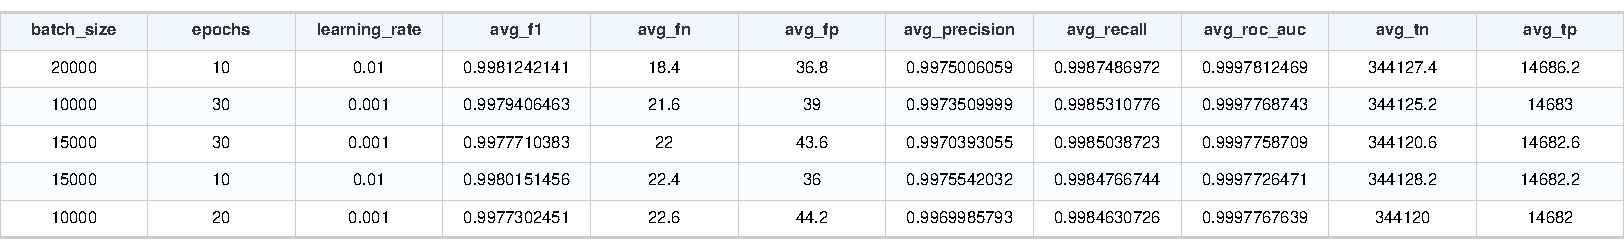
\includegraphics[width=1\textwidth]{./img/modelo/resultados/BINhs98.pdf}
    \caption{Mejores cinco configuraciones de hiperparámetros del modelo de clasificación binaria con una capa oculta de 98 neuronas ($2n$).}
    \label{fig:BINhs98}
\end{figure}

La matriz de confusión de la mejor configuración de hiperparámetros obtenida en el Modelo de Clasificación Binaria de 49 neuronas (MCB98), es la que se muestra en la Figura \ref{fig:MC_ENT_MCB98}.

\begin{figure}[H]
    \centering
    \includegraphics[width=0.5\textwidth]{./img/modelo/matrices_confusion/MC_ENT_MCB98.png}
    \caption{Matriz de confusión de la mejor configuración de hiperparámetros obtenida en el MCB98 durante la fase de búsqueda.}
    \label{fig:MC_ENT_MCB98}
\end{figure}



Estos resultados no son definitivos, puesto que no se está evaluando la posibilidad de que el modelo haya sufrido sobreajuste incluso utilizando validación cruzada. Para obtener resultados reales del desempeño del modelo, se realizan pruebas, también conocidas como test, en las que se obtienen las métricas del modelo al recibir datos que no ha visto nunca. Este proceso y sus resultados se comentan en el capítulo \ref{cap.test} como parte de la fase de evaluación de CRISP-DM.


\subsection{Comparación de las arquitecturas seleccionadas de los modelos de clasificación binaria} \label{sec:comp.BIN}
En esta sección se comaparan los resultados obtenidos entre las tres arquitecturas propuestas. Una vez comparadas, se desarrolla una posible explicación para comprender los resultados de los experimientos.

Para comprender mejor los resultados globales de los experimentos, se han recogido en la Figura \ref{fig:BINtop5}, las 5 configuraciones de hiperparámetros con mayor \textit{Recall} independientemente de su arquitectura.

\begin{figure}[H]
    \centering
    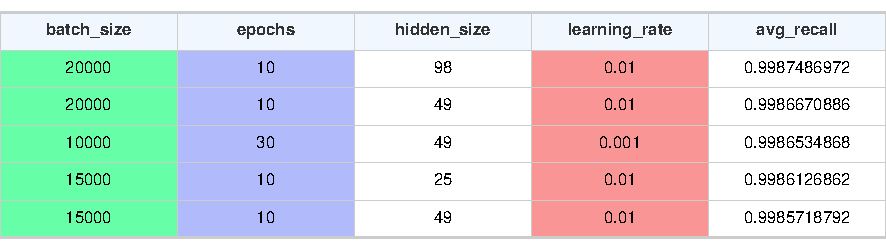
\includegraphics[width=0.85\textwidth]{./img/modelo/resultados/BINtop5.pdf}
    \caption{Mejores cinco configuraciones de hiperparámetros del modelo de clasificación binaria.}
    \label{fig:BINtop5}
\end{figure}

El problema para el que ha sido diseñado el modelo no presenta una relación lineal tras transformar los datos como se explica en el capítulo \ref{cap.ent-datos} \nameref{cap.ent-datos}. Por este motivo, se esperaba que el modelo con un tamaño de capa oculta mayor fuese capaz de converger mejor, tal y como se comenta en \ref{sec:VIBIN98}.

Al observar los datos de la figura \ref{fig:BINtop5}, se puede apreciar que puntualmente, la mejor arquitectura ha sido la que tenía un tamaño de ventana oculta igual a 98. Cabe destacar que, la diferencia entre los valores de \textit{recall} de los cinco mejores experimentos es muy pequeña y puede que se deba a factores externos, como el estado de la máquina en el momento en el que se entreno al modelo, o la inicialización aleatoria de los pesos. Por este motivo, los resultados pueden variar si se realizan los mismos experimentos.

Ente los mejores resultados de los experimentos, detaca la presencia de la arquitectura con un tamaño de capa oculta igual al número de parámetros de entrada del modelo. Tal y como se comenta en las secciones anteriores, esta es la arquitectura más equilibrada. Gracias a este equilibrio ha sido capaz de ajustar sus pesos mejor que el rseto de arquitecturas para configuraciones de hiperparámetros diferentes.

Al aumentar el número de épocas del entrenamiento de los modelos, estos tienden a sobreajustar los pesos. Este sobreajuste implica que el modelo obtiene unas métricas excepcionalmente positivas durante los experimentos. Sin embargo, aunque los valores de las métricas son muy positivos en los experimentos realizados, sorprende que el número de épocas del 80 \% de las 5 mejores configuraciones, es el menor de los valores con los que se han realizado los experimentos para el hiperparámetro \textit{epochs}. Estos resultados reflejan que la probabilidad de que el modelo haya sobreajustado sus pesos es muy baja. Posiblemente, el uso de la validación cruzada que penaliza el sobreajuste de los pesos de los modelos, como se explica en secciones anteriores, sea el responsable de que los experimentos con un número de épocas más elevado hayan obtenido unos resultados peores.

Finalmente, es destacable que el \textit{learning rate} de la mayoría de los 5 mejores experimentos del global de las arquitecturas tenga el valor más alto de los que se han probado. Esto puede interpretarse de manera positiva o negativa.
En el mejor de los casos, un \textit{learning rate} alto muestra que los datos están bien estructurados y que el optimizador y las arquitecturas son robustos frente a valores altos de \textit{learning rate},
En el peor de los casos, la convergencia se realiza rápidamente pero de manera inestable, los resultados dependan en gran medida de los valores iniciales de los pesos o se este sobreajustando el modelo. Este último caso es el más improbable debido a las técnicas utilizadas que se han descrito y a los resultados analizados en el párrafo anterior.

Para conocer el verdadero desempeño del modelo y determinar si ha sufrido sobreajuste de los pesos durante el entrenamiento, se realiza un test con datos que no ha visto el modelo durante el entrenamiento. Estas pruebas y análisis se describen en el capítulo \ref{cap.test} \nameref{cap.test}. Si los resultados obtenidos de estos test son similares a los resultados obtenidos de los experimentos, significa que el modelo converge correctamente hacia una solución real. En caso de que los resultados obtenidos de los test sean significativamente peores que los obtenidos durante los experimentos, el modelo habrá sobreajustado sus pesos. 



\section{Selección de modelos de clasificación multiclase}
En esta sección se pueden observar los resultados de los experimentos realizados con los posibles valores de los hiperparámetros comentados en la sección \ref{sec:disMUL} \nameref{sec:disMUL}.

Para medir la eficiencia y eficacia del modelo, se han obtenido las métricas derivadas de la matriz de confusión comentadas en la sección \ref{sec:metricas-mul} \nameref{sec:metricas-mul}. El objetivo de este modelo es clasificar intrusiones en redes, ya detectadas en diferentes tipos específicos de ataque enumerados en la sección \ref{sec.tipo-ataques} para facilitar una respuesta adecuada. Aunque una clasificación incorrecta puede afectar la eficiencia de la mitigación, las consecuencias no son tan catastróficas como en el caso de falso negativo del modelo de clasificación binaria. Sin embargo, la precisión en la identificación del tipo de ataque sigue siendo clave para optimizar los recursos y la estrategia de defensa.
Teniendo esto en cuenta, la métrica más importante es \textit{Weifhted F1 score}, ya que como se comenta en el apartado anterior, refleja el impacto relativo de cada clase en el conjunto de datos, resultando especialmente útil para comparar modelos entrenados con datasets desbalanceados.

Otras métricas relevantes que se muestran en las siguientes figuras son:
\begin{itemize}
	\item \textbf{ Macro F1 Score}%: Indica un buen equilibrio entre precisión y \textit{recall} promedio por clase, sin importar su frecuencia, lo que refleja buen rendimiento en todas las clases, incluidas las minoritarias.
	\item \textbf{ Macro Recall}%: Un valor alto significa que el modelo detecta correctamente una alta proporción de instancias reales en cada clase, lo que es crucial para no ignorar clases poco representadas.
	\item \textbf{Macro Precision}%: mide qué proporción de predicciones por clase son correctas. Un valor alto implica que el modelo no clasifica erróneamente otras clases como una clase minoritaria.
\end{itemize}

En la Figura \ref{fig:MULhs25}, se encuentran representadas las cinco mejores configuraciones de hiperparámetros para el modelo de clasificación multiclase con una arquitectura de 25 (n/2) neuronas (MCM25) en la capa oculta. Coinciden con lo esperado tras el análisis de la sección \ref{sec:VIMUL25} para esta arquitectura. La mejor configuración para la arquitectura con la mitad de neuronas en la capa oculta que de parámetros de entrada tiene el modelo, ha sido:
\begin{itemize}
	\item \textbf{\textit{Batch size}}: 64
	\item \textbf{\textit{Epochs}}: 100
	\item \textbf{\textit{Learning rate}}: 0.001
\end{itemize}

\begin{figure}[H]
    \centering
    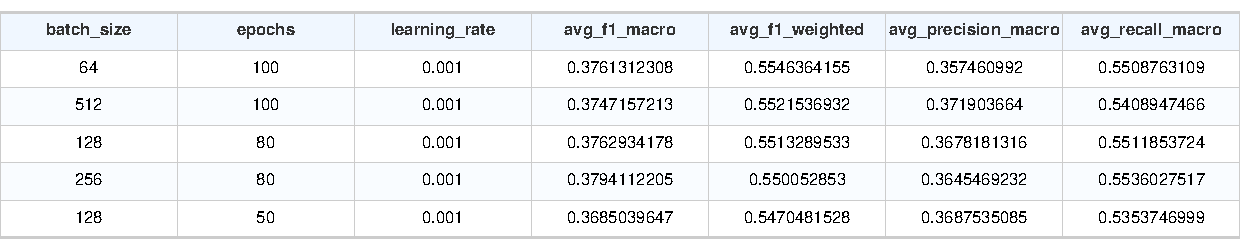
\includegraphics[width=1\textwidth]{./img/modelo/resultados/MULhs25.pdf}
    \caption{Mejores cinco configuraciones de hiperparámetros del modelo de clasificación multiclase con una capa oculta de 25 neuronas.}
    \label{fig:MULhs25}
\end{figure}

Gracias a la matriz de confusión mostrada en la Figura \ref{fig:MC_ENT_MCM25}, es posible visualizar facilmente los resultados obtenidos durante la fase de búsqueda de las mejores configuraciones de los hiperparámetros para el MCM25, ofreciendo una visión aproximada del rendimiento alcanzado.

\begin{figure}[H]
    \centering
    \includegraphics[width=0.8\textwidth]{./img/modelo/matrices_confusion/MC_ENT_MCM25.png}
    \caption{Matriz de confusión de la mejor configuración de hiperparámetros encontrada en la fase de búsqueda para el MCM25.}
    \label{fig:MC_ENT_MCM25}
\end{figure}



La figura \ref{fig:MULhs49}, muestra la representación de las cinco mejores configuraciones de hiperparámetros para el modelo de clasificación multiclase con una arquitectura de 49 (n) neuronas (MCM49) en la capa oculta. Los resultados medios obtenidos son algo peores de lo comentado en el análisis de la sección \ref{sec:VIMUL49} para esta arquitectura. La mejor configuración para la arquitectura con la el mismo número de neuronas en la capa oculta que de parámetros de entrada tiene el modelo, ha sido:
\begin{itemize}
	\item \textbf{\textit{Batch size}}: 256
	\item \textbf{\textit{Epochs}}: 50
	\item \textbf{\textit{Learning rate}}: 0.001
\end{itemize}

\begin{figure}[H]
    \centering
    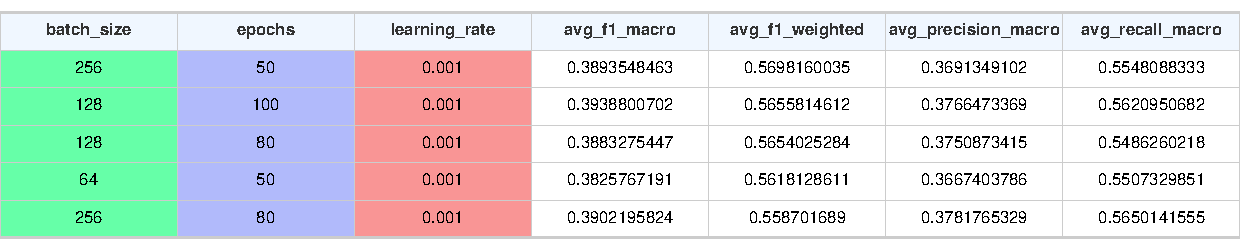
\includegraphics[width=1\textwidth]{./img/modelo/resultados/MULhs49.pdf}
    \caption{Mejores cinco configuraciones de hiperparámetros del modelo de clasificación multiclase con una capa oculta de 49 neuronas.}
    \label{fig:MULhs49}
\end{figure}

Gracias a la matriz de confusión mostrada en la Figura \ref{fig:MC_ENT_MCM49}, es posible visualizar facilmente los resultados obtenidos durante la fase de búsqueda de las mejores configuraciones de los hiperparámetros para el MCM49, ofreciendo una visión aproximada del rendimiento alcanzado.

\begin{figure}[H]
    \centering
    \includegraphics[width=0.8\textwidth]{./img/modelo/matrices_confusion/MC_ENT_MCM49.png}
    \caption{Matriz de confusión de la mejor configuración de hiperparámetros encontrada en la fase de búsqueda para el MCM49.}
    \label{fig:MC_ENT_MCM49}
\end{figure}



En la Figura \ref{fig:MULhs98}, se encuentran representadas las cinco mejores configuraciones de hiperparámetros para el modelo de clasificación multiclase con una arquitectura de 98 (2n) neuronas (MCM98) en la capa oculta. Los resultados obtenidos en esta arquitectura son los que más coindiden con lo explicado en el análisis de la sección \ref{sec:VIMUL98} para esta arquitectura. La mejor configuración para la arquitectura con el doble de neuronas en la capa oculta que de parámetros de entrada tiene el modelo, ha sido:
\begin{itemize}
	\item \textbf{\textit{Batch size}}: 256
	\item \textbf{\textit{Epochs}}: 100
	\item \textbf{\textit{Learning rate}}: 0.001
\end{itemize}

\begin{figure}[H]
    \centering
    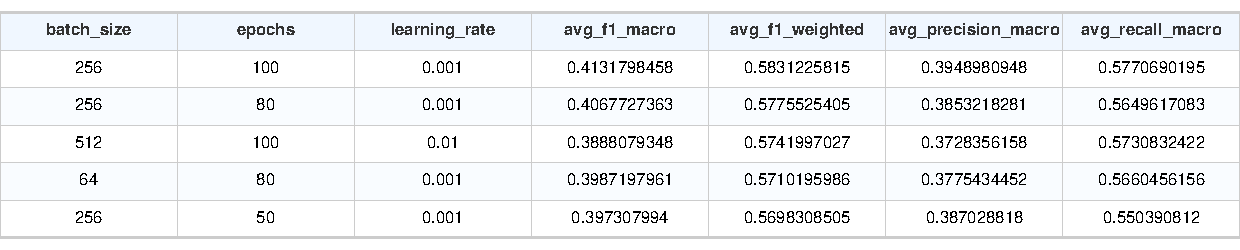
\includegraphics[width=1\textwidth]{./img/modelo/resultados/MULhs98.pdf}
    \caption{Mejores cinco configuraciones de hiperparámetros del modelo de clasificación multiclase con una capa oculta de 98 neuronas.}
    \label{fig:MULhs98}
\end{figure}

Gracias a la matriz de confusión mostrada en la Figura \ref{fig:MC_ENT_MCM98}, es posible visualizar facilmente los resultados obtenidos durante la fase de búsqueda de las mejores configuraciones de los hiperparámetros para el MCM98, ofreciendo una visión aproximada del rendimiento alcanzado.

\begin{figure}[H]
    \centering
    \includegraphics[width=0.8\textwidth]{./img/modelo/matrices_confusion/MC_ENT_MCM98.png}
    \caption{Matriz de confusión de la mejor configuración de hiperparámetros encontrada en la fase de búsqueda para el MCM98.}
    \label{fig:MC_ENT_MCM98}
\end{figure}


Los resultados obtenidos no son definitivos, puesto que no se está evaluando la posibilidad de que el modelo haya sufrido sobreajuste incluso utilizando validación cruzada. Para obtener resultados reales del desempeño del modelo, se realizan pruebas, también conocidas como test, en las que se obtienen las métricas del modelo al recibir datos que no ha visto nunca. Este proceso y sus resultados se comentan en el capítulo \ref{cap.test}.


\subsection{Comparación de las arquitecturas seleccionadas de los modelos de clasificación multiclase}\label{sec:comp.MUL}
En esta sección se comparan los resultados obtenidos entre las tres arquitecturas propuestas. Una vez comparadas, se desarrolla una posible explicación para comprender los resultados de los experimentos.

Para comprender mejor los resultados globales de los experimentos, se han recogido en la Figura \ref{fig:MULtop10}, las 10 configuraciones de hiperparámetros con mayor weightedd f1 score independientemente de su arquitectura.

\begin{figure}[H]
    \centering
    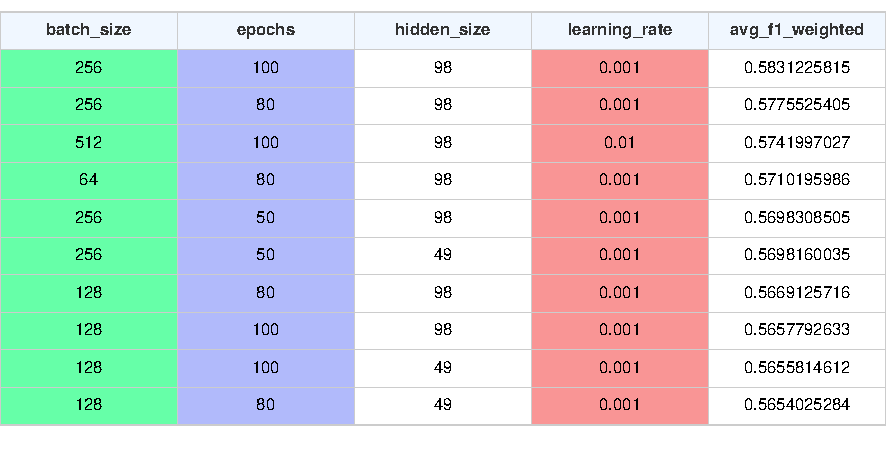
\includegraphics[width=0.85\textwidth]{./img/modelo/resultados/MULtop10.pdf}
    \caption{Mejores diez configuraciones de hiperparámetros del modelo de clasificación multiclase.}
    \label{fig:MULtop10}
\end{figure}

Para poder comparar los resultados de los experimentos del modelo de clasifcación multiclase entre varias arquitecturas, es necesario recoger más combinaciones de hiperparámetros independientemente de las arquitecturas que en la sección \ref{sec:comp.BIN}. Esto denota una gran diferencia ente los resultados de los experimentos del modelo de clasificación multiclase y los resultados del modelo de clasificación binaria. Como se puede observar en la Figura \ref{fig:BINtop5}, los resultados del modelo de clasificación binaria, demuestran que la arquitectura no supone una gran diferencia a la hora de que el modelo converja hacia una solución. En cambio, en los resultados de los experimentos del modelo de clasificación multiclase, la arquitectura con un tamaño de la capa oculta igual al doble del número de entradas del modelo ha sido la dominante.

Los resultados de la Figura \ref{fig:MULtop10} reflejan la complejidad del problema. La hegemonía que presenta la arquitectura con un mayor número de neuronas implica que la relación entre los datos es muy compleja. 

La dificultad del problema que el modelo debe resolver reside en tres características del mismo:

\begin{enumerate}
	\item \textbf{Clases muy desbalanceadas}: Al igual que en el mundo real, los datos utilizados para entrenar el modelo representan varios tipos de intrusiones informáticas a sistemas. Estos tipos de ataques no tienen los mismos objetivos, tal y como se comenta en el capítulo \ref{cap.ent.problema} \nameref{cap.ent.problema}. Como la finalidad de cada tipo de ataque es diferente, el número de ataques de cada clase que se realizan depende de lo que los usuarios que los lanzan deseen conseguir. Esta característica del problema se ve reflejada en la proporción de muestras de cada clase que contiene el \textit{dataset} utilizado. Para comprender la dimensión del problema, de las muestras utilizadas para el entrenamiento del modelo, 31\,052 pertenecen a ataques de tipo Exploits, mientras que solo 109 de las muestras son de tipo \textit{Worms}. Esto implica que el número de muestras que son Exploits es 284 veces mayor que el número de muestras de ataques \textit{Worms}.
	
	\item \textbf{Complejidad para relacionar los datos}: Como se comenta en varias de las secciones anteriores de este capítulo, las relaciones entre los datos que se utilizan para el entrenamiento del modelo no son lineales. La complejidad de los datos implica un mayor número de ajustes por retropropagación en cada época de entrenamiento. Esta característica además de aumentar el coste computacional del entrenamiento y el uso del modelo, requiere de poder ajustar los pesos de la red con mayor precisión que en modelos con una complejidad menor, como es el caso del modelo de clasificación binaria propuesto en este proyecto.
	
	\item \textbf{Número de clases elevado}: Cuanto mayor es el número de clases entre las que debe diferenciar un modelo de clasificación multiclase, mayor número de muestras de cada clase son necesarias para entrenar el modelo y mayor número de situaciones de clasificación erróneas existe. 
	
	El modelo que se ha diseñado debe identificar nueve clases distintas de intrusiones pero debido a la complejidad de obtener datos representativos de cada intrusión, el número de muestras utilizado para entrenar al modelo es de aproximadamente 72\,000. De ese número de muestras, 60\,000 pertenecen solo a tres tipos de clases.
	
	Si se toma de punto de partida la matriz de confusión del modelo de clasificación binaria, existen 4 posibles respuestas del modelo, de las cuales dos de ellas son correctas. Esto implica que, en el hipotético caso, de que el modelo simplemente diese respuestas aleatorias, este daría la respuesta correcta dos de cada cuatro veces, o lo que es lo mismo el 50 \% de las ocasiones. En el caso del modelo de clasificación multiclase, la matriz de confusión tiene 81 posibilidades diferente. De estas posibilidades, solo las que pertenecen a la diagonal principal son respuestas correctas, lo que equivale a nueve respuestas correctas. Aplicando la misma lógica que se ha aplicado para el modelo de clasificación binaria, si el modelo de clasificación multiclase solo diese respuestas de manera aleatoria, acertaría en 9 de cada 81 ocasiones, lo que se traduce en una tasa de acierto del 11,1 \%. Estas tasas de acierto corresponden con la métrica de precisión de cada modelo. Sin embargo, las métricas utilizadas para evaluar que combinación de hiperparámetros es mejor para cada modelo, se ven especialmente afectadas por los falsos negativos y por la clasificación errónea de clases minoritarias, correspondientemente.
\end{enumerate}

Todas estas características comentadas provocan que la matriz de confusión con los datos de entrenamiento del modelo de clasificación multiclase sea la que se muestra en la Figura \ref{fig:MC_ENT_MCM98}. La figura muestra que de las nueve clases que el modelo es capaz de identificar, solo tres de ellas se clasifican con exactitud en la mayoría de las ocasiones. Destaca el número de predicciones erróneas de las clases más minoritarias que han sido clasificadas como clase tres (\textit{Exploits}). Esto se debe al desbalanceo presente en los datos comentado a lo largo de este capítulo.



\chapter{Test}\label{cap.test}
\input{chapters/test}

\chapter{Despliegue}\label{cap.despliegue}
Esta sección aborda la fase de despliegue de los modelos de clasificación binaria y multiclase desarrollados para la detección de conexiones malignas. La fase de despliegue en la metodología CRISP-DM implica la integración de los modelos entrenados en entornos operativos donde sus predicciones contribuyen a la toma de decisiones en tiempo real o en análisis periódicos, facilitando la detección automatizada y escalable de amenazas en redes como se comenta en capítulos anteriores \cite{wirth2000crisp}.

\section{Integración en entornos operativos}

Los modelos de clasificación binaria, orientados a distinguir conexiones malignas de benignas, y los modelos multiclase, diseñados para identificar diferentes categorías de conexiones malignas, deben ser implementados en plataformas que permitan la recepción continua de datos y procesamiento eficiente \cite{baylor2017tensorflow}. 

Para ello, es recomendable desplegarlos mediante APIs o microservicios, asegurando compatibilidad con sistemas de monitorización y respuesta automatizada. En el caso del modelo multiclase, la alta desproporción entre las clases y la naturaleza específica de los datos requieren especial atención en la validación en entorno real, dado que durante la fase de evaluación correspondiente con el capítulo \ref{cap.test} se utiliza el conjunto completo de datos y puede observarse degradación en desempeño frente a la fase de búsqueda \cite{gama2014survey}.

\section{Consideraciones técnicas}

El uso de validación cruzada estratificada durante la fase de búsqueda garantiza la estabilidad en la estimación de rendimiento, pero el despliegue debe contemplar la variabilidad inherente a datos nuevos y no vistos, especialmente en contextos dinámicos como la detección de conexiones malignas \cite{reimers2017optimal}. 

El ajuste adecuado de hiperparámetros, demostrado durante el capítulo \ref{cap.modelos}, debe ser preservado en producción, considerando limitaciones de hardware, latencia y volumen de datos. El control de versiones de los modelos es crucial para realizar actualizaciones y retrocesos en sus configuraciones de pesos, sin afectar a los resultados que devuelva el modelo \cite{peters2017machine}.

\subsection{Patrones arquitectónicos recomendados: Pipeline y Observador}

Para garantizar un despliegue robusto y adaptable de los modelos de clasificación en entornos operativos, lo recomendable es estructurar el sistema empleando patrones arquitectónicos que favorezcan la modularidad, la escalabilidad y la capacidad de respuesta ante eventos. Los patrones \textit{Pipeline} o Filtro Tuberia y Observador destacan como enfoques adecuados para satisfacer los requerimientos funcionales y no funcionales del sistema.

El patrón \textit{Pipeline} permite organizar el procesamiento de datos en una secuencia de etapas independientes, donde cada etapa representa una transformación o acción específica sobre el flujo de datos. Este enfoque favorece la separación de responsabilidades, facilita el mantenimiento, y permite escalar individualmente cada componente. Es particularmente útil para el procesamiento continuo de datos en tiempo real, como en entornos de detección de conexiones malignas \cite{neptune_ml_pipeline}.

Por otro lado, el patrón Observador resulta útil para implementar una arquitectura reactiva, en la cual distintos componentes del sistema (por ejemplo, sistemas de alerta, interfaces de usuario, módulos de registro) pueden suscribirse a los eventos generados por el modelo como la detección de una amenaza. Este patrón facilita una integración flexible entre los modelos de predicción y otros servicios que requieren actuar en función de los resultados generados, sin acoplamiento directo entre ellos \cite{gof_observer_pattern}.

La combinación de ambos patrones permite un diseño desacoplado, extensible y más mantenible, características fundamentales para sistemas de monitorización y respuesta en entornos dinámicos y críticos como la ciberseguridad.


\section{Monitorización y mantenimiento}
Una vez desplegados, los modelos requieren monitorización continua para detectar posibles cambios en la distribución de los datos o en el comportamiento de las conexiones, que puedan afectar el rendimiento del modelo (\textit{data drift} y \textit{concept drift}) \cite{gama2014survey}. En particular, para el modelo multiclase que ha sido entrenado con clases muy desbalanceadas, la monitorización de métricas como el \textit{F1-Weighted} es esencial para asegurar la calidad del diagnóstico en todas las categorías.

El mantenimiento de los modelos, incluye la recopilación de datos reales etiquetados, la reevaluación periódica del modelo y la posible reentrenamiento o ajuste de hiperparámetros para mantener la eficacia en la detección \cite{tsymbal2004problem}.

\section{Impacto y aplicación en el mundo real}

El despliegue efectivo de estos modelos contribuye a mejorar la seguridad en redes mediante la automatización de la detección de conexiones malignas, permitiendo respuestas rápidas y reducción de falsos positivos y negativos. La diferenciación entre múltiples tipos de conexiones malignas aporta un valor añadido para estrategias de mitigación específicas y optimización de recursos \cite{amershi2019software}.

La Figura \ref{fig:despliegue} muestra como podría implementarse de manera básica los modelos desarrollados en un entorno real de un sistema informático.

\begin{figure}[H]
    \centering
    \includegraphics[width=1\textwidth]{./img/despliegue/despliegue.pdf}
    \caption{Ejemplo de despliegue de los modelos en un sistema informático.}
    \label{fig:despliegue}
\end{figure}


\chapter{Tecnologías usadas}\label{cap.tecnologias}
\input{chapters/tecnologias}

\chapter{Seguimiento del proyecto}\label{cap:seguimiento}
\input{chapters/seguimiento}

\chapter{Conclusiones}\label{cap.conclusiones}
\begin{frame}{Conclusiones del proyecto}
	\begin{itemize}
		\item Se han desarrollado con éxito un modelo de clasificación binaria y un modelo de clasificación multiclase, capaces de detectar con gran precisión si una conexión a un sistema es benigna o maligna y de dar un clasificación previa del tipo de intrusión que se está produciendo.
		 \vspace{10mm}
		\item Tanto el MCB como el MCM son modelos basados en una red neuronal de tipo MLP (Perceptrón multicapa).
		 \vspace{10mm}
		\item Para el entrenamiento y la evaluación de los modelos se ha utilizado el \textit{dataset} \texttt{NF-UNSW-NB15-v3}, que está constituido por datos de origen semi-sintético.
	\end{itemize}
\end{frame}


%Esto es una cita: \cite{ej}. Tiene que hacer referencia a la etiqueta de un bibitem.

%Esto es un enlace \href{www.enlace.net}{Enlace}

% Esto es una url \url{http://www.uva.es}


\cleardoublepage
\addcontentsline{toc}{chapter}{Bibliografía}
%\renewcommand\bibname{Referencias Web}
 %\begin{thebibliography}{X}

 %\bibitem{velostat} \textit{Velostat}, \\
 %\textsc{ejemplo.com}.
 %\\Recuperado a tal fecha, \\de \href{http://ejemplo.com}
 %\end{thebibliography}
 
%\nocite{*}
\bibliographystyle{unsrt}
\bibliography{bibliografia}


\end{document}
